% Algorithmique I à la HEB-ESI
% ----------------------------------
\documentclass[a4paper,oneside]{book}

% Les styles
% ----------------------------------
% ===============================================================
% Feuille de style LaTeX pour le cours d'algorithmique 1ère à l'ESI
% ===============================================================

% ===================================================
%   Les gros éléments de mise en page
% ===================================================

% Spécifie que les fichiers sources sont codés en UTF8
% http://www.ctan.org/pkg/inputenc
% ----------------------------------------------------
\usepackage[utf8]{inputenc}

% Francisation des textes
% http://en.wikibooks.org/wiki/LaTeX/Internationalization#Babel
% -------------------------------------------------------------
\usepackage[francais]{babel}
\usepackage[T1]{fontenc}		% Permet de taper des accents

% Plus belles polices vectorielles que computer roman
% http://www.tug.dk/FontCatalogue/lmodern/
% -------------------------------------------------------------
\usepackage{lmodern}			

% Régler les marges des pages
% http://www.ctan.org/pkg/geometry
% vmargin: 1cm de plus automatique
% -------------------------------------------------------------
\usepackage[lmargin=3.5cm,rmargin=3.5cm,vmargin=3cm,footskip=4\baselineskip]{geometry}

% Enlever l'indentation de chaque première ligne de paragraphe
% + léger espace entre les paragraphes.
% http://www.ctan.org/pkg/parskip
% -------------------------------------------------------------
\usepackage{parskip}

% Permet d'avoir des couleurs
% usenames et dvipsnames pour noms prédéfinis
% http://www.ctan.org/pkg/xcolor
% -------------------------------------------------------------
\usepackage[usenames,dvipsnames,svgnames,table]{xcolor}

% Permet de barrer, souligner, ...
% Pour barrer : \sout{texte}
% -------------------------------------------------------------
\usepackage[normalem]{ulem}

% Gestion des images.
% http://www.ctan.org/pkg/graphicx
% -------------------------------------------------------------
\usepackage{graphicx}

% Pour disposer du symbole Euro
% -------------------------------------------------------------
\usepackage[official]{eurosym}

% subscript facile
% -------------------------------------------------------------
\newcommand\textsubscript[1]{\ensuremath{{}_{\mathrm{#1}}}}

% Hyperliens et URL
% http://www.ctan.org/pkg/hyperref
% -------------------------------------------------------------
\usepackage{hyperref}
\hypersetup{
  colorlinks = true,  % Colours links instead of ugly boxes
  urlcolor   = blue,  % Colour for external hyperlinks
  linkcolor  = black  % Colour of internal links
}

% Permet d'avoir les numéros de (sub)sections dans la marge
% Tiré de "Latex Howtos" de Sébastien Combéfis
% -------------------------------------------------------------
\makeatletter
\def\@seccntformat#1{\protect\makebox[0pt][r]{\csname the#1\endcsname\quad}}
\makeatother

% Framed permet d'avoir du texte avec une barre à gauche
%\usepackage{framed}
%\colorlet{shadecolor}{gray!50}
%\renewenvironment{leftbar}{%
  %\def\FrameCommand{\textcolor{shadecolor}{\vrule width 1pt} \hspace{10pt}}%
  %\MakeFramed {\advance\hsize-\width \FrameRestore}}%
%{\endMakeFramed}

% Modification du style pour les captions des figures
\usepackage[font=scriptsize,labelfont=sc,position=below]{caption}

% Plus d'options pour les notes/icones en marge
\usepackage{marginnote}
\reversemarginpar

% Pour un plus beau style pour le titre de chapitre
\usepackage[Lenny]{fncychap}

% Pour avoir Ovalbox
\usepackage{fancybox}

% Un grand contrôle sur l'aspect des listes
% Note: bizarrement, \setlist ne fonctionne pas (\itemize avec options non plus) 
% (clash avec un autre package ?)
% -------------------------------------------------------------
\usepackage{enumitem}
\setdescription{font=\sffamily\bfseries, style=nextline, leftmargin=*}
% Environnement liste, alternative à itemize, plus aéré.
\newlist{liste}{itemize}{3}
\setlist[liste]{label=$\triangleright$,leftmargin=8mm,itemsep=1mm}

% Permet d'avoir des références plus lisibles 
% ex: cf. figure 1 page suivante.
% http://www.ctan.org/pkg/varioref
% -------------------------------------------------------------
\usepackage[french]{varioref}

% Gestion de l'entête et du pied de page
% http://www.ctan.org/pkg/fancyhdr
% -------------------------------------------------------------
\usepackage{fancyhdr}
\setlength{\headheight}{13pt} 
\fancyhf{} % Enlever tout
\renewcommand{\headrulewidth}{0pt} % pas de ligne en entête
\fancyfoot[C]{\textcolor{gray}{---\ \thepage\ ---}}
\fancyhead[R]{\ifnum\value{chapter}>0 \textcolor{gray}{\up{\leftmark}} \fi}
\fancypagestyle{plain}{				% Redéfinir le style plain
	\fancyhf{} 						% Enlever tout
	\fancyfoot[C]{\textcolor{gray}{---\ \thepage\ ---}}
	\renewcommand{\headrulewidth}{0pt} % pas de ligne en entête
}


% ===================================================
%   Commandes et environnements
% ===================================================

% Met en évidence un ou des paragraphes
% titre en gras encadré + croix
% cf. http://tex.stackexchange.com/questions/33078/frame-with-only-crosses-in-two-opposite-corners
\newenvironment{Emphase}[2][]{%
	\section*{\ifthenelse{\not\equal{#1}{}}{\marginnote{\includegraphics[width=25px]{icon/#1}}[2pt]}{}\ovalbox{\normalsize\textbf{#2}}}
	\vspace{-10mm}
	{\color{gray}\par\hfill\rlap{\kern-0.5cm\rule{1cm}{0.4pt}\kern-0.2cm\rule[-0.8cm]{0.4pt}{1cm}}}%
    \vskip-\baselineskip
}{
	{\color{gray}\par\kern-0.8cm\hskip-0.25cm\rule{0.4pt}{1cm}\kern-0.2cm\rule[0.2cm]{1cm}{0.4pt}\par}
	\smallskip
}

% Pour mettre une icone en marge
% Utilisation: \marginicon{nomIcone}
% L'icone doit être présente dans le dossier icon
% dans un format reconnu (pas de gif)
\newcommand{\marginicon}[1]{
	\marginnote{\includegraphics[width=25px]{icon/#1}}[8pt]
}

% Affiche un cadre ovale coloré autour de texte, coloré aussi et en sansserif.
% Pour encadré numéro d'exercice, de tutoriel, ....
% -------------------------------------------------------------
\newcommand{\Cadre}[1]{{\sffamily\Ovalbox{#1}}}

% Pour un exercice avec numérotation automatique
\newcounter{exercicenum}[chapter]
\setcounter{exercicenum}{0}
\newenvironment{Exercice}[1]{%
	\refstepcounter{exercicenum}%
	%\renewcommand{\Currentlabel}{\arabic{chapter}.\theexercicenum}% Pour référence dans la solution
	\vspace{-2mm}
	\subsection*{\normalsize{\color{MidnightBlue}\Cadre{\theexercicenum}}\quad{\sffamily\bfseries#1}}
	\vspace{-2mm}
	}{%
	}
	
% Citation en début de chapitre
\newenvironment{Exergue}{%
	\begin{quote}
	\itshape
	}{
	\end{quote}
	\vskip2\baselineskip
	}

% Permet d'avoir plusieurs colonnes
% Utilisé dans les tableaux pour avoir un contrôle fin des |
\usepackage{multicol}

% Pour les tableaux
% ------------------
\usepackage{hhline} % Permet une gestion fine des barres horizontales 
% Aucune udée de l'intérêt pour les 3 lignes suivantes
\makeatletter
\newcommand\arraybslash{\let\\\@arraycr}
\makeatother{}
\setlength\tabcolsep{1mm} % aére le texte dans les cases de tableau
      % Style principal pour le bouquin
% Adaptation du package algorithmicx pour écrire les algorithmes
% du cours de logique à l'ESI

\usepackage{algpseudocode}		% Perme d'écrire des algorithmes
%\usepackage{algorithm}			% Pour des algorithmes flottants

% ==============================================================
% pseudocode et Pseudocode
% ==============================================================

\newenvironment{pseudo}{%
	\begin{minipage}{0.95\linewidth}
	\begin{sffamily}
	\begin{algorithmic}[0]
	\small
}{%
	\end{algorithmic}
	\end{sffamily}
	\end{minipage}
}
\newcommand{\cadre}[1]{%
	\fcolorbox{gray}{gray!10}{%
		\begin{minipage}{0.97\linewidth}#1\end{minipage}%
	}%
	\smallskip
}
\usepackage{environ} % Merci à astalavista pour ce truc :)
\NewEnviron{Pseudocode}{%
	\cadre{
		\begin{pseudo}
			\BODY
		\end{pseudo}
	}
}
\newcommand{\pseudocode}{\textsf}

% ==============================================================================
% Le code suivant permet d'avoir des lignes verticales pour délimiter les blocs. 
% cf: http://tex.stackexchange.com/questions/52473/is-it-possible-to-have-connecting-loop-lines-like-algorithm2e-in-algorithmic
% J'ai changé la ligne (plus grosse et grise)
% ==============================================================================

% --- Définitions techniques pour avoir les lignes
\makeatletter
\definecolor{rulecolor}{gray}{0.7} % This is the vertical rule that is inserted
\def\therule{\makebox[\algorithmicindent][l]{\hspace*{.4em}{\color{rulecolor}\vrule height .75\baselineskip width 0.05em depth .25\baselineskip}}}%

\newtoks\therules% Contains rules
\therules={}% Start with empty token list
\def\appendto#1#2{\expandafter#1\expandafter{\the#1#2}}% Append to token list
\def\gobblefirst#1{% Remove (first) from token list
  #1\expandafter\expandafter\expandafter{\expandafter\@gobble\the#1}}%
\def\LState{\State\unskip\the\therules}% New line-state
\def\pushindent{\appendto\therules\therule}%
\def\popindent{\gobblefirst\therules}%
\def\printindent{\unskip\the\therules}%
\def\printandpush{\printindent\pushindent}%
\def\popandprint{\popindent\printindent}%

% --- Définition des structures qui vont avoir une ligne
% Boucles
\algdef{SE}[WHILE]{While}{EndWhile}[1]
  {\printandpush\algorithmicwhile\ #1\ \algorithmicdo}
  {\popandprint\algorithmicend\ \algorithmicwhile}%
\algdef{SE}[FOR]{For}{EndFor}[1]
  {\printandpush\algorithmicfor\ #1\ \algorithmicdo}
  {\popandprint\algorithmicend\ \algorithmicfor}%
\algdef{SE}[REPEAT]{Repeat}{Until}
  {\printandpush\algorithmicrepeat}[1]
  {\popandprint\algorithmicuntil\ #1}%
% Alternatives
\algdef{SE}[IF]{If}{EndIf}[1]
  {\printandpush\algorithmicif\ #1\ \algorithmicthen}
  {\popandprint\algorithmicend\ \algorithmicif}%
\algdef{C}[IF]{IF}{ElsIf}[1]
  {\popandprint\pushindent\algorithmicelse\ \algorithmicif\ #1\ \algorithmicthen}%
\algdef{Ce}[ELSE]{IF}{Else}{EndIf}
  {\popandprint\pushindent\algorithmicelse}%
\algdef{SE}[SWITCH]{Switch}{EndSwitch}[1]
  {\printandpush\algorithmicswitch\ #1}
  {\popandprint\algorithmicend\ \algorithmicswitch}%
\algdef{C}[SWITCH]{SWITCH}{Case}[1]
  {\popandprint\pushindent\ #1:}%
% Structures
\algdef{SE}[STRUCT]{Struct}{EndStruct}[1]
  {\printandpush\algorithmicstruct\ #1}
  {\popandprint\algorithmicend\ \algorithmicstruct}%
% Classe
\algdef{SE}[CLASS]{Class}{EndClass}[1]
  {\printandpush\algorithmicclass\ #1}
  {\popandprint\algorithmicend\ \algorithmicclass}%
% Bloc customisable
\algdef{SE}[CUSTOM]{Custom}{EndCustom}
  {\printandpush}
  {\popandprint}
% Bloc
\algdef{SE}[BLOC]{Block}{EndBlock}[1]
  {\printandpush \algorithmicblock\ #1}
  {\popandprint \algorithmicend\ \algorithmicblock}
% Module
\algblockdefx[MODULE]{Module}{EndModule}[3]%
  {\printandpush\algorithmicprocedure\ \textproc{#1}(#2)\ifthenelse{\equal{#3}{}}{}{\Gives\ #3}}
  {\popandprint\algorithmicend\ \algorithmicprocedure}
% Méthode
\algblockdefx[METHOD]{Method}{EndMethod}[3]%
  {\printandpush\algorithmicmethod\ \textproc{#1}(#2)\ifthenelse{\equal{#3}{}}{}{\Gives\ #3}}
  {\popandprint\algorithmicend\ \algorithmicmethod}
% Constructeur
\algblockdefx[CONSTR]{Constr}{EndConstr}[2]%
  {\printandpush\algorithmicconstr\ \textproc{#1}(#2)}
  {\popandprint\algorithmicend\ \algorithmicconstr}
% Parties privées/publiques
\algdef{C}[CLASS]{CLASS}{Private}{\popandprint\pushindent\ privé:}%
\algdef{C}[CLASS]{CLASS}{Public}{\popandprint\pushindent\ public:}%
% Signatures de module / méthode / constructeur
\newcommand{\ModuleSign}[3]{\Stmt \algorithmicprocedure\ \textproc{#1}(#2)\ifthenelse{\equal{#3}{}}{}{\Gives\ #3}}
\newcommand{\MethodSign}[3]{\Stmt \algorithmicmethod\ \textproc{#1}(#2)\ifthenelse{\equal{#3}{}}{}{\Gives\ #3}}
\newcommand{\ConstrSign}[2]{\Stmt \algorithmicconstr\ \textproc{#1}(#2)}
  
% ==============================================================================
% Ajouts propres pour la francisation des termes prédéfinis + nouveaux termes
% ==============================================================================
\algnewcommand\algorithmicclass{\textbf{classe}}
\algnewcommand\algorithmicmethod{\textbf{méthode}}
\algnewcommand\algorithmicconstr{\textbf{constructeur}}
\algnewcommand\algorithmicstruct{\textbf{structure}}
\algnewcommand\algorithmicblock{\textbf{bloc}}
\algnewcommand\algorithmicbegin{\textbf{début}}
\algrenewcommand\algorithmicend{\textbf{fin}}
\algrenewcommand\algorithmicprocedure{\textbf{module}}
\algrenewcommand\algorithmicfunction{\textbf{module}}
\algrenewcommand\algorithmicwhile{\textbf{tant que}}
\algrenewcommand\algorithmicfor{\textbf{pour}}
\algrenewcommand\algorithmicrepeat{\textbf{faire}}
\algrenewcommand\algorithmicuntil{\textbf{jusqu'à ce que}}
\algrenewcommand\algorithmicdo{\textbf{faire}}
\algrenewcommand\algorithmicreturn{\textbf{retourner}}
\algrenewcommand\algorithmicif{\textbf{si}}
\algrenewcommand\algorithmicthen{\textbf{alors}}
\algrenewcommand\algorithmicelse{\textbf{sinon}}
\algnewcommand\algorithmicswitch{\textbf{selon que}}

% ==============================================================================
% Ajout de petits éléments de syntaxe non existants
% ==============================================================================
\newcommand{\In}{\ensuremath{\downarrow}}
\newcommand{\Out}{\ensuremath{\uparrow}}
\newcommand{\InOut}{\In{}\Out{}}
\newcommand{\Gets}{\ensuremath{\gets}\ }
\newcommand{\Gives}{\ \ensuremath{\rightarrow}{}}
\newcommand{\K}[1]{\textbf{#1}} % Keyword
\newcommand{\Decl}{\LState}
\renewcommand{\Return}{\LState\algorithmicreturn\ }
\newcommand{\Open}{\LState\textbf{ouvrir}\ }
\newcommand{\Close}{\LState\textbf{fermer}\ }
\newcommand{\Read}{\LState\textbf{lire}\ }
\newcommand{\Readf}{\LState\textbf{lire}\ }
\newcommand{\Write}{\LState\textbf{afficher}\ }
\newcommand{\Writef}{\LState\textbf{écrire}\ }
\newcommand{\Empty}{\LState}
\newcommand{\Stmt}{\LState}
\newcommand{\Let}{\LState}
\newcommand{\Error}{\LState\textbf{erreur}\ }
% Les commentaires
\algrenewcommand{\algorithmiccomment}[1]{{\small\hskip1em// #1}}
\newcommand{\LComment}{\Empty\hskip-1em\Comment}
\newcommand{\RComment}{\hfill\Comment}
% Pour indenter une ligne
\newcommand{\Indent}{\expandafter\hskip\algorithmicindent\relax}
% Pour une continuation de ligne (2x indenté)
\newcommand{\Suite}{\Stmt\Indent\Indent}

% ==============================================================================
% Modifications de style
% ==============================================================================
\algrenewcommand\textproc{\textit} % Nom de module en italique plutôt qu'en small caps
   % Définition pour les algorithmes

% Identité de l'école
% ----------------------------------
\newcommand{\ecole}{Haute École de Bruxelles}
\newcommand{\entite}{École Supérieure d'Informatique}
\newcommand{\entiteadresse}{Rue Royale, 67 – 1000 Bruxelles}
\newcommand{\entitesite}{www.heb.be/esi}
\newcommand{\entitetel}{02/219.15.46}
\newcommand{\entitemail}{esi@heb.be}
\newcommand{\etude}{Bachelor en Informatique}

% Identité de l'AA
% ----------------------------------
\newcommand{\ue}{DEV2}
\newcommand{\cours}{Algorithmique II}

% Éléments temporels : année - prof
% ----------------------------------
\newcommand{\annee}{2014}

\newcommand{\auteura}{L. Beeckmans}
\newcommand{\auteurb}{M. Codutti}
\newcommand{\auteurc}{G. Cuvelier}
\newcommand{\auteurd}{E. Levy}
\newcommand{\auteure}{F. Servais}
\newcommand{\contact}{mcodutti@heb.be}
\newcommand{\ladate}{\today}

% Index (attendre qu'il soit suffisament rempli)
% ----------------------------------
%\usepackage{makeidx} % pour générer un index
%\makeindex

% Les différentes parties du document
% -----------------------------------
\begin{document}
% =======================================================
% Syllabus de Logique 1ère - Début du document
% =======================================================

% =======================================================
% Page de garde
% =======================================================

\thispagestyle{empty}

% haut-gauche

\includegraphics[scale=0.45]{image/logo-esi}
\begin{minipage}[t]{7cm}
\vspace{-6.5\baselineskip}
\sffamily
\large\textbf{\ecole\\\entite}
\\\vspace{3.5mm}\\
\large\entiteadresse\\\entitetel{} – \entitemail
\end{minipage}
%
% haut-droit
\begin{minipage}[t]{5cm}
\vspace{-6.5\baselineskip}
\sffamily
\raggedleft
\large\textbf{\etude}
\end{minipage}


% centre
\vfill
\begin{center}
\sffamily
\Huge\cours
\bigskip\\
\Large\ue\ -- \annee
\end{center}
\vfill

%bas
Activité d'apprentissage enseignée par :
\begin{center}
\itshape 
\begin{tabular}{*{5}{p{2.2cm}}}
À définir\dots
%\auteura & \auteurb & \auteurc & \auteurd & \auteure \\
%\auteurf & \auteurg & \auteurh & \auteuri & \auteurj \\
\end{tabular}
\end{center}

% =======================================================
% 2ème page : licence, infos de version, ...
% =======================================================

\clearpage
\thispagestyle{empty}

\vfill

Ce syllabus a été écrit à l'origine par M. Monbaliu
à une époque où le cours s'appelait 
\og\ Logique et techniques de programmation \fg.
Il a ensuite été adapté par Mme~Leruste, M.~Beeckmans et M.~Codutti.
Qu'ils en soient tous remerciés.
Nous remercions également tous ceux qui ont contribué à son amélioration
grâce à leur lecture attentive et leurs remarques. 

\bigskip
Document produit avec \LaTeX.
\\Version du \today.

\vfill


\includegraphics[width=25mm]{image/cc-gris}
\\
Ce document est distribué sous licence 
\\Creative Commons Paternité - Partage à l'Identique 2.0 Belgique 
\\(http://creativecommons.org/licenses/by-sa/2.0/be/).
\\Les autorisations au-delà du champ de cette licence
\\peuvent être obtenues à \entitesite{} - \texttt{\contact}.
\pagestyle{fancy}

% =======================================================
% Table des matières
% =======================================================
\setcounter{tocdepth}{1}
\tableofcontents{}


%========================
\chapter{L'orienté objet}
%=========================

	\marginicon{objectif}
	Dans ce chapitre, nous présentons les bases de la programmation orientée
	objet. Nous commençons par expliquer les motivations qui ont amené ce
	type de programmation avant d'entrer dans le vif du
	sujet en explicitant le concept
	d'\textit{encapsulation}. Les autres piliers de
	l'orienté objet (\textit{héritage} et
	\textit{polymorphisme}) ne seront pas vus cette année.

%===================
\section{Motivation}
%====================

	Depuis son apparition, la puissance de l'ordinateur
	n'a cessé de croitre exponentiellement. Les tâches qui
	lui sont confiées ont fait de même. Ainsi les programmes à écrire sont
	de plus en plus gros et de plus en plus complexes.
	
	Face à la complexité, la démarche est toujours la même~: découper le
	problème en sous-problèmes (qui peuvent à leur tour être découpés) ce
	qui permet

	\begin{liste}
		\item 
			d'attaquer chaque problème séparément en évitant la
			surcharge cognitive ;
		\item 
			de répartir le travail entre plusieurs personnes ;
		\item 
			de pouvoir réutiliser du travail déjà produit si un sous-problème est
			déjà apparu dans le cadre d'un autre problème ;
		\item 
			de produire un code plus lisible car s'exprimant avec
			des termes de plus haut niveau, 
			plus proches du problème à résoudre.
			Ainsi, là où un tri devra être fait, 
			on trouvera le mot «~trier~» qui fera référence 
			à la partie de code qui s’occupe du tri. 
			Cela va dans le sens d’une plus grande «~abstraction~» du code~: 
			un code qui s’éloigne du langage simpliste 
			compris par le processeur pour s’approcher de la
			pensée humaine et des termes du problème à résoudre.
	\end{liste}
	
	Les langages de programmation ont suivi cette approche en permettant
	toujours plus d’abstraction. Dans le cours d'algorithmique de DEV1, on vous a
	présenté la notion de module qui permet de découper la tâche à réaliser
	en sous-tâches ainsi que la notion de structure qui permet de regrouper
	des données. Il s'agit là de deux approches	dissociées. 

	C'est cette lacune que se propose de combler
	l'orienté objet~: permettre de définir des
	\textbf{objets} (composés de \textbf{données} et
	\textbf{d'instructions}) qui sont proches du problème
	à résoudre. Cela va permettre une meilleure lisibilité et une plus
	grande concision du code. Ainsi on pourra définir les notions de date,
	d'employé, de fournisseur, de plateau de jeu, de pion,
	de livre, d'emprunteur, de carte à jouer, de chambre,
	de réservation, de vol, de produit, de stock, de ristourne, de facture,
	de panier d'achats, de compte en banque, de banque, de
	client, de portefeuille d'actions\dots

%==========================
\section{La notion d'objet}
%==========================

	\subsection{Définition}
	%-----------------------
	
		\marginicon{definition}
		Un \textbf{objet}%
		\footnote{%
			Les définitions sont tirées du livre de Cardon et
			Dabancourt (cf. bibliographie)
		}
		est une entité logicielle qui~:
	
		\begin{liste}
		\item 
			a une \textbf{identité~}; c'est-à-dire que nous pouvons
			identifier un objet par un nom (tout comme une variable possède un
			nom).
		\item 
			est capable de sauvegarder un \textbf{état}, c'est à
			dire un ensemble d'informations dans des variables
			internes;
		\item 
			répond à des \textbf{messages} précis en déclenchant des activations
			internes appropriées qui peuvent changer l'état de
			l'objet. Ces opérations sont appelées des
			\textbf{méthodes}. Ce sont des fonctions liées à des objets et qui
			précisent le \textbf{comportement} de ces objets.
		\end{liste}

	\subsection{État}
	%-----------------

		\marginicon{definition}
		Un objet contient de l'information, des données qui
		définissent son état.

		\textbf{Exemples}	
		\begin{liste}
		\item 
			Pour un produit, l'état peut être~:
			l'intitulé du produit, son code barre, son prix\dots 
		\item 
			Pour un employé, on peut avoir~: son nom, son prénom, son adresse, sa
			date d'embauche, son salaire mensuel, sa fonction, son
			téléphone\dots
		\item 
			Une carte à jouer a une couleur et une valeur.
		\item 
			L'état d'une date est le jour du
			calendrier qu'elle représente.
		\item 
			L'état d'une heure est le moment de la
			journée qu'elle représente.
		\end{liste}

		L'état d'un objet est mémorisé via des
		variables qu'on appelle des \textit{attributs}.

	\subsection{Attributs}
	%----------------------

		\marginicon{definition}
		Les \textbf{attributs} d'un objet sont
		l'ensemble des informations se présentant sous forme
		de variables et permettant de représenter l'état
		d'un objet.

		Nous verrons plus loin la syntaxe précise 
		pour définir les attributs d'un objet.

		\textbf{Exemples}
		\begin{liste}
		\item 
			L'intitulé d'un produit peut être
			représenté par une chaine. C'est également le cas des
			nom(s) et prénom(s) d'un employé.
		\item 
			La date d'embauche peut être représentée par un «~objet
			date~» (une date est rarement un type primitif du langage utilisé). Un
			attribut d'un objet peut être lui même un objet.
		\item 
			Un moment de la journée peut aussi être un objet représenté par trois
			entiers\footnote{Toutefois, on verra que ce n'est
			peut-être pas la meilleure solution.}~: les heures, les minutes et les
			secondes (en supposant qu'on désire une précision de
			l'ordre de la seconde).
		\item 
			L'adresse d'un employé peut être
			représentée par une seule chaine mais également par un «~objet
			adresse~» (qui contiendrait~: une rue, un numéro, un code postal\dots).
		\end{liste}

		\marginicon{attention}
		\textbf{Remarque}\textbf{~: }Certaines parties de
		l'état peuvent évoluer au fil du temps.
		D'autres parties sont immuables. 
		Ainsi l'adresse d'une personne peut changer
		mais pas sa date de naissance.

		\begin{Emphase}{Exercices - attributs}
			\marginicon{exercice}
			\vskip-\baselineskip
			\begin{enumerate}
				\item 
					Quel(s) attribut(s) prendriez-vous pour représenter
					(l'état d') une date ?
				\item 
					Et pour un dé à 6 faces ?
				\item 
					Et pour un produit de magasin ?
				\item 
					Et pour une télévision ?
					(on peut en trouver vraiment beaucoup !)
			\end{enumerate}
		\end{Emphase}

	\subsection{Comportement}
	%-------------------------

		\marginicon{definition}
		Le \textbf{comportement} d'un objet est défini par
		l'ensemble des messages ou requêtes auxquels il peut répondre.

		Pour ce faire, il exécute un module qui pourra
		éventuellement retourner une information à l'émetteur
		du message.
		
		Les messages peuvent interroger l'objet, le modifier,
		lui demander d'agir sur son environnement (afficher du
		texte, modifier un fichier\dots). 

		\textbf{Exemples}
		\begin{liste}
		\item
			Quels «~messages~» peut-on envoyer à une date ? 
			On peut lui demander (entre autres) :
			\begin{liste}
			\item
				des informations sur le jour du mois, le mois, l'année,
				le jour de la semaine ;
			\item
				si elle est antérieure ou non à une autre date ;
			\item
				si elle fait partie d'une année bissextile ;
			\item
				le nombre de jours qui la sépare de la fin de l'année ;
			\item 
				de passer au jour suivant, à la semaine suivante\dots
			\end{liste}
		\item 
			Et pour un stock de produits ? On peut 
			\begin{liste}
			\item
				lui demander la quantité disponible d'un produit donné ;
			\item
				lui annoncer l'arrivée d'une quantité
				donnée d'un produit donné ;
			\item
				lui indiquer qu'un produit n'existe
				plus (à retirer du stock) ;
			\item 
				lui demander d'enlever une certaine quantité
				d'un produit du stock.
			\end{liste}
		\item
			Et pour un employé ? On peut
			\begin{liste}
			\item 
				lui demander son adresse, son salaire ou sa fonction\dots
			\item 
				augmenter son salaire ;
			\item 
				le changer de fonction ;
			\item 
				le licencier 
				(penser à prévoir une date de départ dans l'état !).
			\end{liste}
		\item 
			Pour un moment de la journée on peut demander s'il se
			situe le matin ou pas\dots	
		\end{liste}

		\begin{Emphase}{Exercices - comportement}
			\marginicon{exercice}
			\vskip-\baselineskip
			\begin{enumerate}
			\item
				Quel comportement voyez-vous pour un téléviseur ?
			\item
				Et pour un produit de magasin ?
			\end{enumerate}
		\end{Emphase}

	\subsection{Méthode}
	%--------------------
	
		\marginicon{definition}
		Un message lance l'exécution d'un
		module appelé \textbf{méthode} dans le jargon de
		l'orienté objet.

		\textbf{Exemples}
		\begin{liste}
		\item
			Pour permettre à une date de passer au jour suivant, nous allons définir
			une méthode qui incrémente le jour du mois en tenant compte
			d'un possible basculement au mois suivant ou à
			l'année suivante.
		\item
			Pour calculer le bénéfice d'un produit, nous allons définir
			une méthode qui, à partir du prix d'achat et du prix de vente,
			calcule le bénéfice.
		\item 
			Pour permettre à un moment d'indiquer
			s'il est le matin ou pas, nous allons définir une
			méthode comme celle-ci (nous verrons plus tard comment
			l'associer aux objets)
	
			\medskip
			\begin{Pseudocode}
				\LComment On suppose que 'heure' est un des attributs utilisés
				\LComment pour représenter l'état (le moment dans la journée)
				\Method{estMatin}{}{booléen}
					\Return heure < 12 \RComment on considère que midi est situé l'après-midi
				\EndMethod
			\end{Pseudocode}
			
			\medskip
			Cet exemple devrait vous sembler familier à deux exceptions près
	
			\begin{liste}
				\item
					on utilise le mot «~\pseudocode{méthode}~» en lieu et place de
					«~\pseudocode{module}~» ;
				\item
					les attributs (l'heure ici) ne sont pas passés en paramètre.
					Une méthode appartient à un objet et connait
					les attributs de cet objet. 
					Nous verrons plus loin la syntaxe précise.
			\end{liste}
		\end{liste}

		\begin{Emphase}{Exercices - méthodes}
			\vskip-\baselineskip
			\marginicon{exercice}
			\begin{enumerate}
			\item 
				Dans le comportement d'un téléviseur, on retrouve
				«~éteindre~» et «~allumer~». 
				À quoi ressemblerait le code de ces méthodes ?
			\item 
				Écrivez la méthode qui permet de passer au jour suivant.
			\item 
				Écrivez la méthode qui calcule 
				le bénéfice réalisé lors de la vente d'un produit.
			\end{enumerate}
		\end{Emphase}

	\subsection{Activer un comportement}

		Pour activer un comportement d'un objet, 
		il faut lui envoyer un message 
		(ou dit autrement, appeler une de ses méthodes). 
		La syntaxe que nous allons utiliser 
		(c'est la plus courante) est la notation pointée.

		\begin{Pseudocode}
			\Stmt nomObjet.nomMéthode()
		\end{Pseudocode}

		\medskip\textbf{Exemple}~:
		Supposons que le nom «~maintenant~» 
		désigne un objet contenant un moment de la journée 
		(on verra comment réaliser cela). 
		Si on veut savoir si on est le matin, on peut écrire

		\begin{Pseudocode}
			\If{maintenant.estMatin()}
				\Stmt ...
			\EndIf
		\end{Pseudocode}

		\begin{Emphase}{Exercice – activer un comportement}
			\marginicon{exercice}
			Écrire la portion de code qui allume une télévision 
			(désignée par «~maTélévision~») 
			et puis l'éteint aussitôt après.		
		\end{Emphase}

	\subsection{Les paramètres d'un comportement}

		Activer un comportement revient à appeler une méthode de
		l'objet. Souvent il est nécessaire
		d'envoyer à l'objet des informations
		complémentaires pour préciser notre demande ce qui se fait via
		l'utilisation des paramètres.

		\textbf{Exemple}~:
		Si on veut modifier le salaire d'un employé, 
		il faut que notre message contienne le nouveau salaire. 
		Autrement dit, 
		il faut communiquer ce nouveau salaire à la méthode 
		de changement du salaire.
		Ce qui donne la méthode suivante~:

		\begin{Pseudocode}
			\Method{modifierSalaire}{nouveauSalaire~: entier}{}
				\Stmt salaire \Gets nouveauSalaire
			\EndMethod
		\end{Pseudocode}

		\begin{Emphase}{Exercices – paramètres du comportement}
			\vskip-\baselineskip
			\marginicon{exercice}
			\begin{enumerate}
			\item 
				Prenons un objet représentant un produit de magasin. 
				Nous supposerons qu'un produit a un \textit{numéro}, 
				un  \textit{libellé}, un \textit{prixAchat}, 
				un \textit{prix de vente} et une \textit{quantitéEnStock}
				Donnez les \textbf{entêtes} des méthodes suivantes 
				qui permettent de~:
				\begin{liste}
				\item 
					obtenir le prix de vente
				\item 
					calculer le bénéfice
				\item 
					donner la quantité restant en stock
				\item 
					dire si le produit est en rupture de stock.
				\end{liste}
						
			\item 
				Prenons un objet représentant une date du calendrier grégorien. 
				Donnez les entêtes des méthodes suivantes qui permettent de~:
				\begin{liste}
				\item
					demander le nom du jour correspondant (par exemple "lundi", "mardi"\dots)
				\item 
					savoir si une date est antérieure à une autre
				\item 
					connaitre le nombre de jours (absolu) séparant deux dates.
				\end{liste}
					
			\item 
				Utilisation. Soit deux dates $date1$ et $date2$ ; écrivez la
				portion de code qui utilise les méthodes ci-dessus pour
				\begin{liste}
					\item 
						vérifier quelle date précède l'autre;
					\item 
						calculer le nombre de jours d'écart entre ces deux
						dates.
				\end{liste}
			\end{enumerate}
		\end{Emphase}
	
%=========================
\section{L'encapsulation}
%=========================

	Un objet possède un état qui est représenté par des attributs. 
	Les bonnes pratiques de la programmation orientée objet préconisent
	fortement que les attributs d'un objet soient
	invisibles en dehors de l'objet. 
	Ils ne pourront être accédés qu'au travers 
	du comportement de l'objet, 
	c'est-à-dire via ses méthodes.
	
	\clearpage
	\marginicon{definition}
	\textbf{%
		Lorsque les détails de l'implémentation
		d'un objet sont masqués aux autres objets, on dit
		qu'il y a \textbf{encapsulation} des données et du
		comportement des objets.
	}
	
	Pourquoi une telle recommandation ? 
	Le but est de garantir la cohérence de l'état de l'objet. 
	Si on pouvait accéder directement à un attribut 
	(et donc le modifier), 
	on pourrait y mettre une valeur incohérente. 
	Par exemple, on pourrait dire que les minutes d'un moment 
	valent -3 ou 75 ou encore que le jour d'une date est 32 !
	
	Dès lors, il nous faudra préciser pour chaque \textbf{membre} 
	(attributs et méthodes) d'un objet s'il est
	\textbf{privé} (inconnu de l'extérieur) ou
	\textbf{public} (connu de l'extérieur). 
	
	Le bon usage impose que tous les attributs soient rendus privés 
	et que les méthodes restent publiques. 
	Toutefois, on pourra trouver également des méthodes privées. 
	Ce sera notamment le cas si plusieurs méthodes d'un objet 
	ont une partie commune ; 
	il sera intéressant de la \textit{factoriser}, 
	c-à-d en faire une méthode privée (ex~: un calcul de maximum).
	
	Puisqu'un attribut est privé,
	il est courant pour chacun des attributs de rencontrer 
	une méthode destinée à connaitre la valeur de cet attribut 
	et une autre qui permet de la modifier.

	\subsection{Accesseur et mutateur}
	%----------------------------------
	
	\marginicon{definition}
	
	\textbf{Accesseur}%
	\footnote{On utilise aussi souvent le mot anglais «~getter~».}%
	~: méthode dont le but est de fournir la valeur d'un attribut.

	\textbf{Mutateur}%
	\footnote{On utilise aussi souvent le mot anglais «~setter~»}%
	~: méthode dont le but est de modifier la valeur d'un attribut.

	Par convention, 
	ces méthodes sont nommées \pseudocode{getNom} et 
	\pseudocode{setNom} où «~nom~» est le nom de l'attribut%
	\footnote{%
		Pour un attribut booléen, 
		on pourra préférer \pseudocode{estNom} ou \pseudocode{isNom} 
		au lieu de \pseudocode{getNom}. 
	}
	Par facilité, on utilisera parfois le terme «~accesseur~»
	pour désigner à la fois les «~accesseurs~» et les «~mutateurs~».

	\textbf{Exemple}~:
	Écrivons l'accesseur et le mutateur pour l'attribut 
	«~heure~» d'un moment de la journée.

	\begin{Pseudocode}
		\Method{getHeure}{}{entier}
			\Return heure
		\EndMethod
	\end{Pseudocode}

	\begin{Pseudocode}
		\Method{setHeure}{uneHeure~: entier}{}
			\Stmt heure \Gets uneHeure
		\EndMethod
	\end{Pseudocode}

	\subsection{Que faire si le paramètre est invalide ?}
	%-----------------------------------------------------
	
	Dans l'exemple précédent, 
	que se passerait-il si le paramètre \pseudocode{uneHeure} vaut 25 ? 
	Une valeur aberrante serait affectée à l'attribut \pseudocode{heure}.

	Dans le cas de paramètres invalides, 
	la plus mauvaise solution est de ne rien faire. 
	Le programme continuerait en croyant que tout s’est bien
	passé et il court à la catastrophe. 
	Il est préférable qu’un programme s'interrompe 
	plutôt que de fournir une mauvaise réponse. 

	Dans certains langages (comme le C), 
	l’usage est que chaque module retourne un entier indiquant 
	s'il y a eu une erreur (et laquelle). 
	L’inconvénient est que le module appelant n’est pas
	obligé de tenir compte de l’erreur.

	Les \textbf{exceptions} sont un mécanisme du même genre 
	mais qui oblige à fournir un code de traitement de l’erreur. 
	Il ne sera pas étudié en première année%
	\footnote{%
		En tout cas pas au cours d'algorithmique 
		mais vous étudierez cette notion au cours de Java.%
	}.

	Cette année, nous nous contenterons d'indiquer
	clairement dans nos codes qu'il s'agit d'une situation anormale 
	via la primitive \pseudocode{erreur} qui arrête le déroulement du
	programme avec une courte explication du problème.

	La syntaxe que nous allons retenir est

	\begin{Pseudocode}
		\Stmt \K{erreur} "explication de l'erreur"
	\end{Pseudocode}

	Ce qui donne~:	
	
	\begin{Pseudocode}
		\Method{setHeure}{uneHeure~: entier}{}
			\If{uneHeure < 0 OU uneHeure > 23}
				\Stmt \K{erreur} "heure invalide"
			\EndIf
			\Stmt heure \Gets uneHeure
		\EndMethod
	\end{Pseudocode}

	%\medskip
	%\textbf{Remarque}~: 
	%Accéder à la valeur d’un attribut ne pose pas 
	%de problème de validité. 
	%Alors pourquoi rendre l’attribut complètement privé 
	%plutôt que de n’empêcher que des modifications directes 
	%(une sorte d’attribut en \textit{lecture seule}) ? 
	%Cela permet de changer de façon transparente la représentation des données. 
	%Nous y reviendrons plus loin.

	%\begin{Emphase}{Exercice - encapsulation}
		%\marginicon{exercice}
		%Sans le savoir, vous avez déjà défini des accesseurs et des 
		%mutateurs pour le téléviseur. 
		%Lesquels ? 
		%En suivant la convention de nom pour les accesseurs et les mutateurs, 
		%quels noms auraient-ils dû porter ?
	%\end{Emphase}

%====================================================
\section{La notion de classe et d'instance}
%=====================================================

	Pour pouvoir utiliser des objets nous allons devoir les définir
	(expliciter leur état et leur comportement). 
	Cette définition est commune à tous les objets similaires. 
	Par exemple tous les moments ont un même comportement 
	et un même type d'état 
	(des heures, des minutes et des secondes).
	
	\marginicon{definition}
	\textbf{Une \textbf{classe} est un ensemble d'objets qui ont en
	commun les mêmes méthodes et qui partagent les mêmes types
	d'attributs.}

	Une \textbf{instance}%
	\footnote{%
		Vous pouvez considérer les termes
		«~instance de classe~» et «~objet~» comme synonymes.
	}
	d'une classe est un objet particulier
	d'une classe qui peut activer les méthodes de la
	classe et qui a des valeurs particulières pour ses attributs.

	On peut établir le parallélisme avec les types de base que vous avez
	déjà vus. Définir une classe revient à définir un nouveau type de
	données. En gros, on peut dire qu'un \textbf{objet
	est à une classe ce qu'une variable est à un type}.
	
	Comprenons bien que les objets d'une même classe ont le
	même «~type~» d'état mais pas le même état proprement
	dit. Deux objets «~moment~» représentent tous deux un moment 
	(heures, minutes, secondes) de la journée mais pas (forcement) 
	le même ! Ils auront donc les mêmes attributs mais
	avec des valeurs différentes !
	
	\subsection{Définition d'une classe}
	%------------------------------------
	
		Nous devons d'abord définir une classe avant de pouvoir
		en instancier les objets que nous voulons utiliser. Précisons la
		syntaxe utilisée pour définir une classe

		\begin{Pseudocode}
			\Class{NomDeLaClasse}
				\Private
					\LComment liste des attributs (donc privés par convention)
				\Public
					\LComment liste des méthodes publiques
				\Private
					\LComment liste des méthodes privées
			\EndClass
			\LComment Par souci de lisibilité, on pourra indiquer uniquement 
			les entêtes des
			\LComment méthodes et donner le code complet des méthodes à 
			la suite de la classe.
		\end{Pseudocode}

		\textbf{Exemple}~: 
		la classe Moment qui représente un moment de la journée.

		\begin{Pseudocode}
			\Class{Moment}
				\Private
					\Decl heure~: entier
					\Decl minute~: entier
					\Decl seconde~: entier
				\Public
					\MethodSign{getHeure}{}{entier}
					\MethodSign{getMinute}{}{entier}
					\MethodSign{getSeconde}{}{entier}
					\MethodSign{setHeure}{uneHeure~: entier}{}
					\MethodSign{setMinute}{uneMinute~: entier}{}
					\MethodSign{setSeconde}{uneSeconde~: entier}{}
					\MethodSign{estMatin}{}{booléen}
			\EndClass
			\Empty
			\Method{estMatin}{}{booléen}
				\Return heure < 12
			\EndMethod
			\LComment + les accesseurs et les mutateurs		
		\end{Pseudocode}

	\subsection{Instanciation d'une classe}
	%---------------------------------------
	
		«~Instancier~» signifie créer un objet d'une classe.
		Cela s'écrit avec l'instruction
		\pseudocode{nouveau}. 
		Pour lui donner un nom, 
		on l'assigne à une variable déclarée du type de la
		classe.

		\begin{Pseudocode}
			\Decl nomObjet~: nomClasse 
			\RComment déclaration de l'objet
			\Let nomObjet \Gets \K{nouveau} nomClasse() 
			\RComment instanciation de l'objet
		\end{Pseudocode}

		Dans ce cours de Logique, nous adopterons le fait que 
		les noms des paramètres soient différents de ceux des 
		attributs (on préconisera d’imaginer des noms variés tels 
		que uneDate, maDate, laListe, autreObjet…), ce qui évitera 
		toute ambigüité (entre minuscule et majuscule par exemple).

		\textbf{Exemple}~: pour créer un moment de la journée.
		
		\begin{Pseudocode}
			\Module{test}{}{}
				\Decl midi~: Moment
				\RComment déclaration
				\Let midi \Gets \K{nouveau} Moment()
				\RComment instanciation
				\Stmt midi.setHeure( 12 )
				\RComment mutateur
				\Stmt midi.setMinute( 0 )
				\RComment " "
				\Stmt midi.setSeconde( 0 )
				\RComment " "
				\If{midi.estMatin()}
					\Write "Midi est considéré comme
					étant encore le matin"
				\Else 
					\Write "Midi est considéré comme
					étant l'après-midi"
				\EndIf
			\EndModule
		\end{Pseudocode}

		%Remarquez qu'il y a une différence importante entre les
		%objets et les types de bases. Lorsqu'on déclare une
		%variable d'un type de base, cela alloue
		%automatiquement un espace mémoire pour cette variable.
		%C'est différent avec les objets. La déclaration
		%n'entraine qu'une réservation mémoire
		%pour une «~référence~» vers un objet. Celui-ci
		%n'existe pas encore. Il sera créé (et sa mémoire
		%allouée) via une instruction spécifique (\pseudocode{nouveau}). On
		%parle de variable «\textit{~dynamique~}». Le nom est alors~une
		%«~référence~» vers l’objet. Les avantages de cette dissociation seront
		%évidents lorsque nous parlerons de la notion de \textit{constructeur}.

		%Après la déclaration, on a~:
		%\begin{center}
		%\begin{tabular}{m{2.2089999cm}}
		%\centering\arraybslash  midi\\\hline
		%\multicolumn{1}{|m{2.2089999cm}|}{\centering\arraybslash
		%\itshape rien}\\\hline
		%\end{tabular}
		%\end{center}

		%Après l'instanciation (ou création), on a~:
		%\begin{center}
		%\begin{tabular}{m{2.578cm}m{2.261cm}|m{3.162cm}|}
		%\centering  midi &
		%\multicolumn{1}{m{2.261cm}}{~
		%} &
		%\multicolumn{1}{m{3.162cm}}{\centering\arraybslash
		 %Moment}\\\hhline{-~-}
		%\multicolumn{1}{|m{2.578cm}|}{~
		%} &
		%\centering \sffamily $\rightarrow$ &
		%\centering\arraybslash  heure = ?\\\hhline{-~~}
		%~
		 %&
		%~
		 %&
		%\centering\arraybslash  minute = ?\\
		%~
		 %&
		%~
		 %&
		%\centering\arraybslash  seconde = ?\\\hhline{~~-}
		%\end{tabular}
		%\end{center}
		
		%Remarquez qu'il n'y a pas d'initialisation par défaut, pour le moment.

		%Après l'action des mutateurs, on a~:
		%\begin{center}
		%\begin{tabular}{m{2.578cm}m{2.261cm}|m{3.162cm}|}
		%\centering  midi &
		%\multicolumn{1}{m{2.261cm}}{~
		%} &
		%\multicolumn{1}{m{3.162cm}}{\centering\arraybslash
		 %Moment}\\\hhline{-~-}
		%\multicolumn{1}{|m{2.578cm}|}{~
		%} &
		%\centering \sffamily $\rightarrow$ &
		%\centering\arraybslash  heure = 12\\\hhline{-~~}
		%~
		 %&
		%~
		 %&
		%\centering\arraybslash  minute = 0\\
		%~
		 %&
		%~
		 %&
		%\centering\arraybslash  seconde = 0\\\hhline{~~-}
		%\end{tabular}
		%\end{center}

		\begin{Emphase}{Exercices – classe et instance}
			\vskip-\baselineskip
			\marginicon{exercice}
			\begin{enumerate}
				\item 
					Pour les produits, vous avez déjà écrit les attributs et les en-têtes des
					méthodes. Regroupez le tout en une classe \pseudocode{Produit}
					\textbf{en respectant les notations que vous venez de voir.}
				\item 
					Écrivez un module qui affiche le prix d'achat d'un produit, son prix 
					de vente hors TVA et son prix de vente TVA comprise.
			\end{enumerate}		
		\end{Emphase}

%==========================
\section{Les constructeurs}
%===========================

	L'encapsulation nous permet de contrôler
	l'état de l'objet et de
	l'empêcher de tomber dans un état invalide. Mais
	qu'en est-il de l'état de départ ?
	Est-il valide ?
	
	Il serait bon, lorsqu'on crée un objet (via
	\pseudocode{nouveau}) de pouvoir indiquer l'état
	initial de l'objet et que cet état puisse être validé.
	C'est le rôle précis des constructeurs.
	
	\marginicon{definition}
	Un \textbf{constructeur} est une méthode particulière permettant
	d'initialiser les attributs d'un
	objet lors de sa création effective. Elle porte le même nom que sa
	classe et ne retourne pas de valeur.
	
	Il peut y avoir plusieurs constructeurs ce qui permet
	d'offrir plusieurs possibilités d'indiquer l'état initial de
	l'objet. Toutefois, nous limiterons au maximum le nombre 
	de constructeurs dans une classe.
	
	Remarquez que cela demande de définir plusieurs méthodes 
	qui portent le même nom.
	
	\marginicon{definition}
	
	\textbf{Surcharge} : 
	le fait de définir plusieurs méthodes portant le même nom.
	On doit pouvoir les différencier via leurs paramètres.

	\textbf{Exemple}~:
	Écrivons des constructeurs pour un moment de la journée~:

	\begin{Pseudocode}
		\Class{Moment}
			\Private
				\LComment pas de changement
				\Decl heure~: entier
				\Decl minute~: entier
				\Decl seconde~: entier
			\Public
				\ConstrSign{Moment}{uneHeure, uneMinute, uneSeconde~: entiers}
				\ConstrSign{Moment}{uneHeure, uneMinute~: entiers}
				\RComment 0 seconde par défaut
				\ConstrSign{Moment}{uneHeure~: entier}
				\RComment initialiser à une heure pile
				\Empty
				\LComment pas de changement au niveau des méthodes~:
				\MethodSign{getHeure}{}{entier}
				\MethodSign{getMinute}{}{entier}
				\MethodSign{getSeconde}{}{entier}
				\MethodSign{setHeure}{uneHeure~: entier}{}
				\MethodSign{setMinute}{uneMinute~: entier}{}
				\MethodSign{setSeconde}{uneSeconde~: entier}{}
				\MethodSign{estMatin}{}{booléen}
		\EndClass
		\end{Pseudocode}

	\begin{Pseudocode}
		\Constr{Moment}{uneHeure, uneMinute, uneSeconde~: entiers}
			\Stmt setHeure(uneHeure)
			\Stmt setMinute(uneMinute)
			\Stmt setSeconde(uneSeconde)
		\EndConstr
		
		\Empty
		\Constr{Moment}{uneHeure, uneMinute~: entiers}
			\Stmt setHeure(uneHeure)
			\Stmt setMinute(uneMinute)
			\Stmt setSeconde(0)
		\EndConstr
		
		\Empty
		\Constr{Moment}{uneHeure~: entier}
			\Stmt setHeure(uneHeure)
			\Stmt setMinute(0)
			\Stmt setSeconde(0)
		\EndConstr
			
		\Empty
		\LComment + les accesseurs, les mutateurs et les autres méthodes
	
	\end{Pseudocode}

	Contrairement à ce qu'on peut trouver dans certains langages, 
	comme Java par exemple, nous n'autorisons pas ici d'appel 
	d'un constructeur d'une classe \pseudocode{A} dans un autre constructeur 
	de cette même classe \pseudocode{A}.
	
	Par contre, il est courant en logique qu'un constructeur 
	appelle les mutateurs afin d'effectuer les tests sans 
	avoir à les dupliquer.
	Mais c'est une démarche que vous éviterez de faire dans
	des langages comme Java par exemple 
	(cela vous sera expliqué plus tard).
	
	Lorsqu'on instancie un objet, les paramètres
	qu'on donne déterminent le constructeur qui est
	effectivement utilisé pour initialiser l'état de
	l'objet.

	\textbf{Exemple}~: Instancions quelques moments de la journée.
	
	\begin{Pseudocode}
		\Let heureDépart \Gets \K{nouveau} Moment(14, 23, 56)
		\Let heureLever \Gets \K{nouveau} Moment(9, 30)
		\Let heureGouter \Gets \K{nouveau} Moment(17)
	\end{Pseudocode}

	Le fait qu'un objet est instancié via la primitive
	\pseudocode{nouveau} et pas implicitement à la déclaration permet de
	postposer sa construction effective au moment où
	l'état initial qu'on veut lui donner
	sera connu (ce qui peut résulter d'un calcul). On est
	ainsi assuré que tous les objets manipulés sont valides ce qui permet
	d’éviter les situations où une méthode fait des dégâts suite à la
	manipulation d’un objet invalide.
	
	\begin{Emphase}{Exercices - constructeur}
		\vskip-\baselineskip
		\marginicon{exercice}
		\begin{enumerate}
			\item {
				Écrivez un ou des constructeur(s) pour un \pseudocode{Produit}}
			\item {
				Adaptez le module écrit plus haut pour qu'il affiche le prix hors TVA
				puis le prix TVA comprise du produit numéro 105176 (Lego réveil figurine policier)
				au prix d'achat de 25\euro, au prix de vente de 30\euro et 
				dont il y a 10 exemplaires en stock.}
		\end{enumerate}
	\end{Emphase}

%================================================
\section{Du choix de la représentation de l'état}
%=================================================

	Lorsqu'on définit une classe, il faut choisir les
	attributs qui vont permettre de représenter l'état des
	objets. Cela peut paraitre immédiat mais il n'en est
	rien.
	
	\textbf{Exemple}
		
	Pour un moment de la journée, nous avons choisi
	d'utiliser trois attributs entiers (les heures, les
	minutes et les secondes). Nous aurions tout aussi bien pu choisir
	d'utiliser un seul entier représentant le nombre de
	secondes écoulées depuis minuit.
	
	Ces deux représentations sont tout-à-fait équivalentes en terme de
	potentiel mais la grande différence est l'efficacité
	du code des méthodes. 
	
	Prenons deux méthodes symptomatiques~: celle qui donne
	l'heure et celle qui compare deux moments de la
	journée. La première est beaucoup plus simple à écrire et plus rapide
	avec la première représentation alors que la seconde méthode est plus
	simple à écrire et plus rapide avec la seconde représentation.
	
	Dès lors, quelle représentation choisir ? Il faut examiner, pour chaque
	représentation possible, le nombre de méthodes qui sont efficaces mais
	aussi imaginer la fréquence de leur utilisation (ce qui est difficile
	et changeant). Heureusement, ce choix n'est pas
	définitif. Si on change d'avis, on peut changer la
	représentation. Il faudra bien sûr réécrire les méthodes de la classe
	mais il ne faudra rien changer au reste du code, c-à-d les lignes du
	code utilisant la classe. C’est d’ailleurs là une des grandes forces de
	la programmation orientée objet.

	\begin{Emphase}{Exercices – représentation de l'état}
		\vskip-\baselineskip
		\marginicon{exercice}
		\begin{enumerate}
			\item 
				Compléter la classe Moment en écrivant la méthode «~getHeure~» et celle
				qui compare deux moments pour les deux représentations imaginées
				ci-dessus.
			\item 
				Écrire le module qui crée deux moments de la journée et vérifie si le
				premier est avant le second. Ce code dépend-il des attributs choisis
				pour définir la classe Moment ?
		\end{enumerate}
	\end{Emphase}

	\marginicon{attention}
	\textbf{Remarque}
	
	Précédemment, nous avons défini un \textbf{accesseur} comme une méthode
	permettant d’accéder à la valeur d’un attribut. Mais c’est au
	développeur de définir quels sont les attributs ; c’est totalement caché
	à l’utilisateur de la classe. On voit donc bien que cette notion
	d’accesseur n’a pleinement de sens qu’en interne, pour le développeur
	de la classe. Pour l’utilisateur il s’agit d’une méthode comme les
	autres.

%=====================================
\section{Quelques éléments de syntaxe}
%=====================================

	Clarifions certaines notations liées aux objets.

	\begin{liste}
		\item
			On peut directement afficher un objet. 
			Cela affiche son état, c'est-à-dire les valeurs de ses attributs.

			\begin{Pseudocode}
				\Decl rendezVous~: Moment
				\Let rendezVous \Gets \K{nouveau} Moment(14, 23, 56)
				\Write rendezVous 
				\RComment affichera 14, 23 et 56 dans un format lisible quelconque
			\end{Pseudocode}
		\item
			De même, on peut directement lire un objet,
			ce qui a pour effet de créer un objet avec un état
			correspondant aux valeurs lues pour ses attributs.

			\begin{Pseudocode}
				\Decl rendezVous~: Moment
				\Read rendezVous
			\end{Pseudocode}
		%\item
			%Un nom d'objet est en fait une \textbf{référence} à
			%l'objet. Ainsi l'affectation ne copie
			%pas l'objet mais sa référence. Au final, nous avons
			%deux noms identifiant le même objet
			%\\
			%\bigskip
			%\begin{Pseudocode}
				%\Decl moment1, moment2~: Moment
				%\Let moment1 \Gets \K{nouveau} Moment(14, 23, 56)
				%\Let moment2 \Gets moment1
				%\RComment moment1 et moment2 désignent le même objet
				%\Stmt moment2.setHeure( 12 )
				%\Write moment1.getHeure() 
				%\RComment affiche 12 !!!
			%\end{Pseudocode}
	
			%\bigskip
	
			%\begin{center}
			%\begin{tabular}{m{2.19cm}m{2.2779999cm}|m{2.975cm}|m{2.34cm}m{2.146cm}}
			%\hhline{-~-~-}
			%\multicolumn{1}{|m{2.19cm}|}{\centering  moment1}
			%&
			%\centering \sffamily $\rightarrow$ &
			%\centering  Heure = \sout{14} 12 &
			%\multicolumn{1}{m{2.34cm}|}{\centering \sffamily
			%$\leftarrow$} &
			%\multicolumn{1}{m{2.146cm}|}{\centering\arraybslash
			 %moment2}\\\hhline{-~~~-}
			%~
			 %&
			%~
			 %&
			%\centering  minute = 23 &
			%~
			 %&
			%~
			%\\
			%~
			 %&
			%~
			 %&
			%\centering  seconde = 56 &
			%~
			 %&
			%~
			%\\\hhline{~~-~~}
			%\end{tabular}
			%\end{center}
	
			%\bigskip
	
		\item 
			Le signe «~=~» peut être utilisé pour comparer deux objets.
			Ils seront considérés comme égaux s'ils sont dans le même état, 
			c'est-à-dire que leurs attributs ont la même valeur.
	\end{liste}
	
	\bigskip
	
	\begin{liste}
		\item {
			\textbf{Un attribut privé n'est pas connu en dehors de la
			classe.}
			
			Précisons~: un attribut privé n'est connu que
			des instances de cette classe, ce qui signifie qu'il
			est également connu par tous les autres objets de la même
			classe.
			
			\smallskip
			\textbf{Exemple}~: 	
			écrivons la méthode qui teste si un moment précède un
			autre (en supposant que l'état est représenté par un
			seul entier, totalSecondes, le nombre de secondes depuis minuit)
			
			\bigskip
			\begin{Pseudocode}
				\Method{estAntérieur}{autre~: Moment}{booléen}
					\Return totalSecondes < autre.totalSecondes
					\LComment c'est équivalent à \K{retourner} totalSecondes < autre.getTotalSecondes()
				\EndMethod
			\end{Pseudocode}
			}
			\bigskip
		\item
			Lorsqu'on déclare un objet, il n'est pas encore créé.
			On peut utiliser la valeur spéciale «~rien~»
			pour indiquer ou tester qu'un objet n'est pas encore créé.
			\\
			\bigskip
			\begin{Pseudocode}
				\Decl moment~: Moment								\RComment moment = rien
				\Let moment \Gets \K{nouveau} Moment( 14, 23, 56 )	\RComment moment ${\neq}$ rien
				\If{moment $\neq$ rien}
					\Let moment \Gets rien							\RComment moment = rien
				\EndIf
			\end{Pseudocode}
	\end{liste}
	
%===============================================	
\section{Représentation modélisée d'une classe}
%===============================================

	Un dessin étant souvent plus lisible qu'un texte, on
	peut représenter graphiquement une classe. Une notation courante est
	celle utilisée en UML\footnote{{Unified
	Modeling Langage. }On vous en parlera plus en détail au cours
	d'Analyse.}. Pour faire simple, une classe est
	représentée par un rectangle composé de 3 zones~: la première pour le
	nom de la classe, la deuxième pour les attributs et la troisième pour
	les méthodes. On indique par un signe «~+~» (resp. «~-~») que le membre
	est public (resp. privé)

	\textbf{Exemple}
	
	\begin{center}
	\begin{tabular}{|m{7cm}|}
	\hline
	\centering\arraybslash \bfseries Moment\\\hline
	{ {}- heure~: entier}
	
	{ {}- minute~: entier}
	
	 {}- seconde~: entier\\\hline
	{ + getHeure() \textsf{$\rightarrow$} entier}
	
	{ + setHeure( uneHeure~: entier )}
	
	{ + avancer1Heure()}
	
	 ...\\\hline
	\end{tabular}
	\end{center}

	Remarquons qu'on indique l'entête des méthodes mais
	pas le code associé. En fonction du niveau de détail désiré, on
	pourrait aussi omettre les paramètres et types de retour.

%=======================================
\section{Un exemple complet~: une durée}
%=======================================

	Examinons un exemple complet pour fixer les notions introduites par ce
	chapitre. Lors de l'apprentissage du pseudo-code, vous
	avez écrit quelques modules manipulant des heures (conversion du format
	HMS en nombre de secondes depuis minuit, conversion inverse, différence
	entre 2 heures, …). Il est souvent utile, lorsqu’on développe un
	algorithme, d’avoir à sa disposition un tel type de données au même
	titre que les types prédéfinis. Faisons-le !
	
	\subsection{Ce que l’on veut vraiment}
	
		Avant tout, il faut bien préciser ce que l’on veut décrire. L’«~heure~»
		est un concept multifacettes. Parle-t-on de l’heure comme moment dans
		la journée ou de l’heure comme représentant une durée ? Dans le premier
		cas, elle ne peut dépasser 24h et la différence entre 2 heures n’a pas
		de sens (ou plus précisément n’est pas une heure, mais une durée !).
		Dans le deuxième cas, on n’a pas ces contraintes. Nous allons ici
		adopter la deuxième approche et pour bien la distinguer, nous allons
		plutôt appeler cela une \textbf{durée}.
	
	\subsection{Le comportement (les méthodes)}
	
		La première question à se poser est celle des services qu’on veut
		fournir, c’est-à-dire des méthodes publiques de la classe. On doit
		pouvoir \textit{construire} une durée. On doit pouvoir connaitre le
		nombre de jours, d’heures, minutes ou secondes correspondant à une durée. On doit
		pouvoir effectuer des calculs avec des durées (addition, soustraction).
		Enfin, on doit pouvoir comparer des durées. Arrêtons-nous là, mais en
		pratique, on pourrait trouver encore bon nombre d’autres méthodes qu’il
		serait intéressant de fournir. Ce qui nous donne jusqu’à présent
		
		\begin{Pseudocode}
			\Class{Durée}
				\Private
					\LComment rien encore
				\Public
					\ConstrSign{Durée}{secondes~: entier}
					\ConstrSign{Durée}{heure, minute, seconde~: entiers}
					\Empty
					\MethodSign{getJour}{}{entier}
					\RComment nb de jours dans une durée
					\MethodSign{getHeure}{}{entier}
					\RComment entier entre 0 et 23 inclus
					\MethodSign{getMinute}{}{entier}
					\RComment entier entre 0 et 59 inclus
					\MethodSign{getSeconde}{}{entier}
					\RComment entier entre 0 et 59 inclus
					\Empty
					\MethodSign{getTotalJours}{}{entier}
					\RComment Le nombre total de jours
					\MethodSign{getTotalHeures}{}{entier}
					\RComment Le nombre total d’heures
					\MethodSign{getTotalMinutes}{}{entier}
					\RComment Le nombre total de minutes
					\MethodSign{getTotalSecondes}{}{entier}
					\RComment Le nombre total de secondes
					\Empty
					\MethodSign{ajouter}{autreDurée~: Durée}{}
					\MethodSign{différence}{autreDurée~: Durée}{Durée}
					\MethodSign{égale}{autreDurée~: Durée}{booléen}
					\MethodSign{plusPetit}{autreDurée~: Durée}{booléen}
			\EndClass
		\end{Pseudocode}
		
		\marginicon{attention}
		\textbf{Quelques remarques}
		\begin{liste}
			\item {
				On a deux constructeurs, ce qui offre plus de souplesse pour initialiser
				un objet. Ceci est un exemple supplémentaire du concept de
				«\textbf{~surcharge~}».}
			\item {
				Faisons bien la distinction entre les méthodes
				\pseudocode{getXXX()} et \pseudocode{getTotalXXX()}. Par
				exemple, la méthode \pseudocode{getMinute()} retourne la valeur
				de la composante «~minutes~» dans une représentation HMS tandis que la
				méthode \pseudocode{getTotalMinutes()} retourne le nombre total
				de minutes entières pour cette durée. Ex~: pour 1h23’12’’,
				\pseudocode{getMinute()} retourne 23 et
				\pseudocode{getTotalMinutes()} retourne 83. Idem avec 
				les jours, les heures	et les secondes.}
			\item {
				Les méthodes \pseudocode{getTotalXXX()} retournent le nombre
				(toujours entier) de XXX contenus dans la durée. Exemple, avec la durée
				0h23’52'’, \pseudocode{getTotalMinutes()}
				retourne 23 et pas 24 (autrement dit, il n’y a pas d’arrondi vers le
				haut).}
			\item {
				Il n’y a pas de \textit{mutateur }(\pseudocode{setXXX()}). Ce qui
				signifie qu’on ne peut pas changer directement la valeur de l’objet
				après son initialisation. On aurait pu en définir mais nous
				n'avons pas jugé utile de le faire dans ce cas
				précis.}
			\item {
				La méthode \pseudocode{ajouter()} ne retourne rien. En effet,
				elle ajoute la durée à l’objet sur lequel est appelée la méthode. C’est
				un choix ; on aurait aussi pu dire que la méthode ne modifie pas
				l’objet mais en retourne un autre qui représente la somme. Dans ce cas,
				on l’aurait plutôt appelée «\pseudocode{~plus( )}~».}
			\item {
				La méthode \pseudocode{différence()}, elle, renvoie toujours une
				durée (positive).}
		\end{liste}
	
	\subsection{La représentation de l'état (les attributs)}
	
		La question suivante est~: «~Comment représenter une durée en interne ?
		». Plusieurs possibilités existent. Par exemple~:	
		\begin{liste}
			\item 
				via le nombre d’heures, de minutes et de secondes
			\item 
				via le nombre total de secondes
			\item 
				via une chaine, par exemple au format «~HH~:MM~:SS~» où HH pourrait
				éventuellement excéder 23.
		\end{liste}
		
		Le premier choix semble le plus évident mais réfléchissons-y de plus
		près. D’une part, pourquoi se limiter aux heures. On pourrait
		introduire un champ ‘\pseudocode{jour}’ (après tout on a bien
		une méthode \pseudocode{getJour()}). 
		
		Quel critère doit vraiment nous permettre de décider ? Il faut une
		représentation qui soit suffisante (tout est représenté) et qui
		permette d’écrire des méthodes lisibles et si possible efficaces
		(c'est-à-dire où le calcul est rapide). Selon ces
		critères, la deuxième représentation est de loin la meilleure. Ce qui
		nous donne
		
		\begin{Pseudocode}
			\Class{Durée}
				\Private
					\Decl totalSecondes~: entier
				\Public
					\LComment idem
			\EndClass
		\end{Pseudocode}
	
	\subsection{L'implémentation}
	
		On est à présent prêt pour écrire le code des méthodes. Ce qui nous
		donne pour la classe dans son entièreté~:
		
		\begin{Pseudocode}
			\Class{Durée}
				\Private
					\Decl totalSecondes~: entier
				\Public
					\ConstrSign{Durée}{secondes~: entier}
					\ConstrSign{Durée}{heure, minute, seconde~: entiers}
					\Empty
					\MethodSign{getJour}{}{entier}
					\RComment nb de jours dans une durée
					\MethodSign{getHeure}{}{entier}
					\RComment entier entre 0 et 23 inclus
					\MethodSign{getMinute}{}{entier}
					\RComment entier entre 0 et 59 inclus
					\MethodSign{getSeconde}{}{entier}
					\RComment entier entre 0 et 59 inclus
					\Empty
					\MethodSign{getTotalHeures}{}{entier}
					\RComment Le nombre total d’heures
					\MethodSign{getTotalMinutes}{}{entier}
					\RComment Le nombre total de minutes
					\MethodSign{getTotalSecondes}{}{entier}
					\RComment Le nombre total de secondes
					\Empty
					\MethodSign{ajouter}{autreDurée~: Durée}{}
					\MethodSign{différence}{autreDurée~: Durée}{Durée}
					\MethodSign{égale}{autreDurée~: Durée}{booléen}
					\MethodSign{plusPetit}{autreDurée~: Durée}{booléen}
			\EndClass
		\end{Pseudocode}

		\begin{Pseudocode}
			\Constr{Durée}{secondes~: entier}
				\If{secondes < 0}
					\Stmt \K{erreur} "paramètre négatif"
				\EndIf
				\Let totalSecondes \Gets secondes
			\EndConstr
			\Empty
			\Constr{Durée}{heure, minute, seconde~: entiers}
				\If{heure < 0 OU minute < 0 OU seconde < 0}
					\Stmt \K{erreur} "un des paramètres est négatif"
				\EndIf
				\Let totalSecondes \Gets 3600*heure + 60*minute + seconde
			\EndConstr
		\end{Pseudocode}

		\begin{Pseudocode}
			\LComment Retourne le nombre de jours dans une 
			représentation JJ/HH:MM:SS
			\Method{getJour}{}{entier}
				\Return totalSecondes DIV (3600*24)
			\EndMethod
			\Empty
			\LComment Retourne le nombre d'heures dans une 
			représentation JJ/HH:MM:SS
			\Method{getHeure}{}{entier}
				\LComment On doit enlever les jours éventuels
				\Return (totalSecondes DIV 3600) MOD 24
			\EndMethod
			\Empty
			\LComment Retourne le nombre de minutes dans une 
			représentation JJ/HH:MM:SS
			\Method{getMinute}{}{entier}
				\LComment On doit enlever les heures éventuelles
				\Return (totalSecondes DIV 60) MOD 60
			\EndMethod
			\Empty
			\LComment Retourne le nombre de secondes dans une 
			représentation JJ/HH:MM:SS
			\Method{getSeconde}{}{entier}
				\LComment On doit enlever les minutes éventuelles
				\Return totalSecondes  MOD 60
			\EndMethod
		\end{Pseudocode}

		\begin{Pseudocode}
		
			\LComment Retourne le nombre entier d’heures complètes
			\Method{getTotalHeures}{}{entier}
				\Return totalSecondes DIV 3600
			\EndMethod
			\Empty
			\LComment Retourne le nombre entier de minutes complètes
			\Method{getTotalMinutes}{}{entier}
				\Return totalSecondes DIV 60
			\EndMethod
			\Empty
			\LComment Retourne le nombre entier de secondes complètes
			\Method{getTotalSecondes}{}{entier}
				\Return totalSecondes
			\EndMethod
		\end{Pseudocode}

		\begin{Pseudocode}
			\Method{ajouter}{autreDurée~: Durée}{}
				\Let totalSecondes \Gets totalSecondes + autreDurée.totalSecondes
			\EndMethod
			\Empty
			\Method{différence}{autreDurée~: Durée}{Durée}
				\Return \K{nouvelle} Durée(valeurAbsolue(totalSecondes - autreDurée.totalSecondes))
			\EndMethod
			\Empty
			\Method{égale}{autreDurée~: Durée}{booléen}
				\Return totalSecondes = autreDurée.totalSecondes
			\EndMethod
			\Empty
			\Method{plusPetit}{autreDurée~: Durée}{booléen}
				\Return totalSecondes < autreDurée.totalSecondes
			\EndMethod
		\end{Pseudocode}
		
		Et c’est tout ! Chaque méthode est très petite. C’est une constante en
		orienté objet~: écrire de petites méthodes qui font chacune une et une
		seule chose bien précise.
	
%%===============================
%\section{Ce qu'on n'a pas vu...}
%%================================

	%Nous n'avons évidemment pas épuisé le sujet de
	%l'orienté objet. 
	%Celui-ci est composé de trois piliers~: l'\textbf{encapsulation},
	%l'\textbf{héritage} et le \textbf{polymorphisme}.
	
	%Nous venons de voir l'essentiel de la partie «~encapsulation~». 
	%Les deux autres notions, plus complexes, 
	%seront abordées au cours de Java 
	%mais également au cours de Logique de deuxième année. 
	%En voici un aperçu~:
	
	%\subsection{L'héritage}
	%%-----------------------
	
		%\marginicon{definition}
		%L’\textbf{héritage} permet de définir une classe 
		%à partir d’une autre qui lui sert de base. 
		%On peut alors
		%\begin{liste}
			%\item étendre son état ;
			%\item augmenter ou modifier son comportement.
		%\end{liste}
		
		%Par exemple, on pourra définir un \pseudocode{Etudiant} à partir
		%de la notion de \pseudocode{Personne}.
		
		%La classe qui sert de point de départ est appelée \textbf{classe de
		%base}, \textbf{classe mère} ou encore \textbf{super-classe}. La classe
		%qu’on définit à partir d’une classe mère est appelée \textbf{classe
		%dérivée}, \textbf{classe fille} ou encore \textbf{sous-classe}.
		
		%Cette notion est un préalable pour le pilier suivant, le
		%\textbf{polymorphisme}.
	
	%\subsection{Le polymorphisme}
	%%-----------------------------
	
		%\marginicon{definition}
		%Le \textbf{polymorphisme} permet d’utiliser un objet fille 
		%en lieu et place d’un objet mère. 
		
		%Exposé aussi brièvement cela peut paraitre futile mais cela
		%permet de construire du code ayant une architecture élégante, robuste
		%et facilement adaptable.

%==================
\section{Exercices}
%==================

	Vous trouverez en annexe, 
	quelques classes que vous pouvez utiliser sans les définir : 
	\pseudocode{Date}, \pseudocode{Moment} et \pseudocode{Durée}
	
%\begin{Exercice}{Un produit}
	%Reprendre la classe \pseudocode{Produit} qui a servi
	%d'exemple. Identifier et écrire les méthodes qui vous
	%paraissent utiles pour une telle classe.
	
	%À partir de là, écrire la classe Stock. Qu'utiliseriez-vous 
	%comme attributs et quelles méthodes vous paraissent utiles pour
	%cette classe ?
%\end{Exercice}

\begin{Exercice}{Une personne}
	Créer une classe \pseudocode{Personne}, une personne étant
	constituée d'un nom, d'un prénom et
	d'une date de naissance. Cette classe utilisera la
	classe \pseudocode{Date}.

	On doit pouvoir construire une personne~:

	\begin{liste}
		\item 
			avec 3 arguments~: le nom (\pseudocode{chaine}), le prénom
			(\pseudocode{chaine}) et la date de naissance de la personne
			(\pseudocode{Date})
		\item 
			avec 2 arguments de type chaine~: le nom et le prénom de la personne; la
			date de naissance est alors initialisée à «\pseudocode{~rien~}»
	\end{liste}

	Écrire aussi tous les accesseurs et mutateurs que vous jugez
	pertinents. Dans un module principal, créer une personne~:

	\begin{enumerate}[label=\alph*)]
		\item 
			avec comme arguments {\textquotedbl}Durant{\textquotedbl} et
			{\textquotedbl}Zébulon{\textquotedbl}
		\item 
			avec comme arguments {\textquotedbl}Durant{\textquotedbl},
			{\textquotedbl}Zébulon{\textquotedbl} et la date de naissance du
			$1^{er}$ février 1989
	\end{enumerate}

	Pour réaliser les constructeurs recevant la date de naissance en
	paramètre, il faudra tester si cette date n’est pas antérieure à la
	date du jour. 
\end{Exercice}

\begin{Exercice}{Anniversaire des personnes}
	À l'aide de la classe \pseudocode{Personne} écrite plus haut,
	écrire un module qui lit des \pseudocode{Personne} (au clavier)
	et affiche les noms et le nombre de celles nées ce mois-ci. On suppose
	que la lecture de «~rien~» indique la fin des données.
\end{Exercice}

%\begin{Exercice}{La classe rectangle (version orientée objet)}
	%Nous avons déjà abordé les rectangles dans le chapitre des variables
	%structurées. Nous reprenons cet exercice sous l’angle de l’orienté
	%objet.

	%Créer une classe \textbf{Rectangle}
	%permettant de définir des rectangles dont les cotés sont parallèles aux
	%axes des coordonnées dans un plan cartésien. Plusieurs représentations
	%sont possibles~:

	%\begin{liste}
		%\item 
			%la position d’un des sommets et les mesures des cotés;
		%\item 
			%les positions de deux sommets opposés;
		%\item 
			%la position du centre et les demi-mesures des cotés, etc.
	%\end{liste}

	%N’hésitez pas à utiliser la structure Point définissant un point dans un
	%plan cartésien.

	%Une fois les attributs choisis, écrire divers constructeurs~:

	%\begin{enumerate}[label=\alph*)]
		%\item 
			%sans arguments~: le rectangle est un carré de coté 1 centré en (0,0)
		%\item
			%avec deux paramètres~: les mesures des cotés horizontaux et verticaux,
			%le rectangle étant centré en (0,0)
		%\item 
			%avec trois paramètres~: la position du coin en haut à gauche (structure
			%Point) et les mesures des cotés horizontaux et verticaux 
		%\item 
			%avec deux paramètres de type Point~: les positions de deux sommets
			%opposés
	%\end{enumerate}

	%Veillez à vérifier la validité des paramètres !

	%Doter ensuite la classe de méthodes permettant~:

	%\begin{enumerate}[label=\alph*)]
		%\item 
			%d’obtenir la position du centre
		%\item 
			%d’obtenir la position du coin inférieur droit
		%\item 
			%de calculer le périmètre du rectangle
		%\item 
			%de calculer la surface du rectangle
		%\item 
			%de déplacer le rectangle en donnant l’amplitude du déplacement au niveau
			%des abscisses et des ordonnées
		%\item 
			%de multiplier les dimensions du rectangle par un facteur $k$, le centre
			%restant au même endroit
		%\item 
			%de faire pivoter le rectangle de 90 degrés autour de son centre
		%\item 
			%de vérifier si un rectangle à une intersection avec un autre rectangle
	%\end{enumerate}
	
%\end{Exercice}

%\begin{Exercice}{Test}

	%Test~: écrire un module TestRectangle en vue de tester le bon
	%fonctionnement de la classe \pseudocode{Rectangle} de l'exercice précédent. Ce module~: 

	%\begin{enumerate}[label=\alph*)]
		%\item 
			%crée un rectangle R1 par défaut
		%\item 
			%crée un rectangle R2 de cotés 5 et 7, et centré en (0,0)
		%\item 
			%crée un rectangle R3 possédant les sommets (-2,3) et (4, -5)
		%\item 
			%affiche la surface de R1 et le périmètre de R2
		%\item 
			%déplace R1 d’une unité vers le bas
		%\item 
			%déplace R2 de 2 unités vers la droite
		%\item 
			%grossit R3 d’un facteur 3
		%\item 
			%effectue une rotation de 90 degrés à R2
		%\item 
			%indique si R2 et R3 possèdent une intersection
	%\end{enumerate}

	%À présent, choisir une autre représentation des attributs et récrire
	%tout le contenu de la classe (très long, courage !).
	%Récrire ensuite le
	%module TestRectangle (très rapide !)
%\end{Exercice}

% ====================================
\chapter{Les tableaux à 2 dimensions}
% ====================================

% ===================
\section{Définition}
% ===================

	\marginicon{definition}
	La \textbf{dimension} d’un tableau est le nombre d’indices qu’on utilise
	pour faire référence à un de ses éléments. Attention de ne pas confondre 
	avec la	taille !
	
	Dans ce qui précède, nous avons introduit les tableaux à une dimension.
	Un seul indice suffisait à localiser un de ses éléments. De nombreuses
	situations nécessitent cependant l’usage de tableaux à deux dimensions.
	Ils vous sont déjà familiers par leur présence dans beaucoup de
	situations courantes : calendrier, grille horaire, grille de mots
	croisés, sudoku, jeux se déroulant sur un quadrillage (damier,
	échiquier, scrabble \dots).

% ====================
\section{Déclaration}
% ====================

	\marginicon{definition}
	Pour déclarer un tableau statique à 2 dimensions, on écrira :

	\begin{Pseudocode}
	\Decl nomTableau : \K{tableau} [ligMin à ligMax, colMin à colMax] de TypeElément
	\end{Pseudocode}
	
	Pour un tableau dynamique, on procédera en deux étapes comme expliqué
	pour les tableaux à une dimension. 
	
	\begin{Pseudocode}
	\Decl nomTableau~: \K{tableau} de TypeElément
	\LComment Le code peut déterminer ici les bornes
	\Let nomTableau \Gets \K{nouveau} \K{tableau} [ligneMin à ligneMax, colMin à colMax] de TypeElément
	\end{Pseudocode}

	où \pseudocode{ligneMin}, \pseudocode{ligneMax}, 
	\pseudocode{colMin} et \pseudocode{colMax} sont des
	expressions entières quelconques.

	On ne se permettra pas en logique de
	combiner les deux types de tableaux, à savoir utiliser la notation
	«~statique~» pour certaines dimensions et «~dynamique~» pour les
	autres.

	Notez qu'un tableau à deux dimensions peut aussi être
	vu comme un tableau à une dimension dont chacun des éléments est
	lui-même un tableau à une dimension.

	\textbf{Exemple} : Soit le tableau déclaré ainsi:

	\begin{Pseudocode}
	\Decl ntabLettres : \K{tableau}[1 à 4, 1 à 5] de caractères
	\end{Pseudocode}

	On peut le visualiser à l’aide d’une grille à 4 lignes et 5 colonnes.

	\begin{center}
	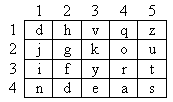
\includegraphics[width=4cm]{image/tab2d-vision-tab2d}
	\end{center}

	Ainsi, la valeur de \pseudocode{tabLettres[3,4]} 
	est le caractère ‘r’. 
	
	La vision «~tableau de tableau~» 
	(ou décomposition en niveaux)
	donnerait :

	\begin{center}
	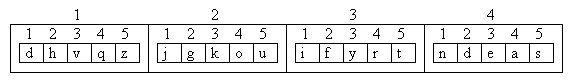
\includegraphics[width=0.9\textwidth]{image/tab2d-vision-tabtab}
	\end{center}

	Dans cette représentation, le tableau \pseudocode{tabLettres} est
	d’abord décomposé à un premier niveau en quatre éléments auxquels on
	accède par le premier indice. Ensuite, chaque élément de premier niveau
	est décomposé en cinq éléments de deuxième niveau accessibles par le
	deuxième indice.
	
	\textbf{Exemple~:} reprenons l'exemple du stock de 10 produits
	qui a servi d'introduction au chapitre sur les tableaux
	mais, cette fois, pour chaque jour de la semaine.
	
	\begin{small}
	\begin{center}
		\begin{tabular}{*{8}{>{\centering\arraybackslash}m{1.5cm}}}
			~ &
			{article1} &
			{article2} &
			{article3} &
			\dots &
			{article8} &
			{article9} &
			{article10}\\
		\end{tabular}	
		\begin{tabular}{|m{1.5cm}|*{7}{>{\centering\arraybackslash}m{1.5cm}|}}
			\hline
			{lundi} & 
			{cpt[1,1]} &
			{cpt[1,2]} &
			{cpt[1,3]} &
			\dots &
			{cpt[1,8]} &
			{cpt[1,9]} &
			{cpt[1,10]}
			\\\hline
			{mardi} &  
			{cpt[2,1]} &
			{cpt[2,2]} &
			{cpt[2,3]} &
			\dots &
			{cpt[2,8]} &
			{cpt[2,9]} &
			{cpt[2,10]}
			\\\hline
			{mercredi} & 
			{cpt[3,1]} &
			{cpt[3,2]} &
			{cpt[3,3]} &
			\dots &
			{cpt[3,8]} &
			{cpt[3,9]} &
			{cpt[3,10]}
			\\\hline
			{jeudi} & 
			{cpt[4,1]} &
			{cpt[4,2]} &
			{cpt[4,3]} &
			\dots &
			{cpt[4,8]} &
			{cpt[4,9]} &
			{cpt[4,10]}
			\\\hline
			{vendredi} & 
			{cpt[5,1]} &
			{cpt[5,2]} &
			{cpt[5,3]} &
			\dots &
			{cpt[5,8]} &
			{cpt[5,9]} &
			{cpt[5,10]}
			\\\hline
			{samedi} & 
			{cpt[6,1]} &
			{cpt[6,2]} &
			{cpt[6,3]} &
			\dots &
			{cpt[6,8]} &
			{cpt[6,9]} &
			{cpt[6,10]}
			\\\hline
			{dimanche} & 
			{cpt[7,1]} &
			{cpt[7,2]} &
			{cpt[7,3]} &
			\dots &
			{cpt[7,8]} &
			{cpt[7,9]} &
			{cpt[7,10]}
			\\\hline
		\end{tabular}
	\end{center}
	\end{small}
	
	\bigskip

	\begin{Pseudocode}
	\LComment Calcule et affiche la quantité vendue de 10 produits
	\LComment pour chaque jour de la semaine (de 1~: lundi à 7~: dimanche).
	\Module{statistiquesVentesSemaine}{}{}
		\Empty
		\Decl cpt~: \K{tableau} [1 à 7, 1 à 10] d’entiers
		\Decl produit, jour~: entiers
		\Empty
		\Stmt initialiser(cpt)
		\Empty
		\LComment Pour chaque jour de la semaine
		\For{jour \K{de} 1 \K{à} 7}
			\Stmt traiterStock1Jour(cpt, jour)
			\For{produit \K{de} 1 \K{à} 10}
				\Write "quantité vendue de produit ", produit, " ce jour ", jour, "~: ", cpt[jour][i]
			\EndFor
		\EndFor	
	\EndModule
	\end{Pseudocode}

	\begin{Pseudocode}
	\LComment Ce module initialise le tableau d'entiers à 0
	\Module{initialiser}{entiers\InOut~: \K{tableau} [1 à 7, 1 à 10] d’entiers}{}
		\Decl i, j~: entiers
		\For{i \K{de} 1 \K{à} 7}
			\For{j \K{de} 1 \K{à} 10}
				\Let cpt[i,j] \Gets 0
			\EndFor
		\EndFor
	\EndModule
	\end{Pseudocode}

	\begin{Pseudocode}
	\LComment Ce module effectue le traitement du stock pour une journée.
	\Module{traiterStock1Jour}{cpt~\InOut: \K{tableau} [1 à 7, 1 à 10] d’entiers, jour~: entier}{}
		\Decl numéroProduit, quantité~: entiers
		\Write "Introduisez le numéro du produit~:"
		\Read numéroProduit
		\Empty
		\While{numéroProduit > 0}
			\Empty
			\Write "Introduisez la quantité vendue~:"
			\Read quantité
			\Empty
			\Let cpt[jour,numéroProduit] \Gets cpt[jour,numéroProduit] + quantité
			\Empty
			\Write "Introduisez le numéro du produit~:"
			\Read numéroProduit
			\Empty
		\EndWhile
	\EndModule
	\end{Pseudocode}
	
	Pour plus d'exemples, allez faire un tour à la section \vref{algo:Tab2D}.

% ============================================
\section{La troisième dimension (et au-delà)}
% ============================================

	Certaines situations complexes nécessitent l'usage de
	tableaux à 3 voire plus de dimensions.

	\marginicon{definition}
	Pour déclarer un tableau statique à $k$ dimensions, on écrira :

	\begin{Pseudocode}
	\Decl nomTableau : \K{tableau} [ bMin\_1 à bMax\_1, \dots, bMin\_k à bMax\_k] de TypeElément
	\end{Pseudocode}

	où chaque paire de bornes \pseudocode{bMin\_i}~et
	\pseudocode{bMax\_i} limite l’indice correspondant 
	à la $i^{ème}$	dimension du tableau.
	
	
% ================================================
\section{Parcours d'un tableau à deux dimensions}
\label{algo:Tab2D}
% ================================================

Comme nous l'avons fait pour les tableaux à  une dimension,
envisageons le parcours des tableaux à deux dimensions 
(n lignes et m colonnes).

Déclaration d'un tableau statique~:

\begin{Pseudocode}
	\Decl tab~: tableau [1 à n, 1 à m] de T
\end{Pseudocode}

Déclaration d'un tableau dynamique~:

	\begin{Pseudocode}
	\Decl tab~: \K{tableau} de T
	\Let tab \Gets \K{nouveau} \K{tableau} [1 à n, 1 à m] de T
	\end{Pseudocode}

Commençons par des cas plus simples 
où on ne parcourt qu'une seule des dimensions 
puis attaquons le cas général.

\subsection{Parcours d'une dimension}

On peut vouloir ne parcourir qu'une seule ligne du tableau.
Si on parcourt la ligne $l$, on visite les cases 
$(l,1)$, $(l,2)$, \dots, $(l,m)$.
L'indice de ligne est constant et c'est l'indice de colonne qui varie.

\begin{center}
$l$
\begin{tabular}{|*{5}{>{\centering\arraybackslash}m{0.3cm}|}}
\hline
\ & \ & \ & \ & \  \\
\hline
\cellcolor{gray!25}\ & \cellcolor{gray!25}\ & \cellcolor{gray!25}\ & \cellcolor{gray!25}\ & \cellcolor{gray!25}\  \\
\hline
\ & \ & \ & \ & \  \\
\hline
\end{tabular}
\end{center}

Ce qui donne l'algorithme :

\begin{Pseudocode}
	\LComment{Parcours de la ligne $l$ d'un tableau à deux dimensions}
	\For{c de 1 à m}
		\Stmt traiter tab[l,c]
	\EndFor
\end{Pseudocode}

Retenons~: pour parcourir une ligne, on utilise une boucle sur les colonnes. 

Symétriquement, on pourrait considérer le parcours de la colonne $c$
comme avec l'algorithme suivant.

\begin{Pseudocode}
	\LComment{Parcours de la colonne $c$ d'un tableau à deux dimensions}
	\For{l de 1 à n}
		\Stmt traiter tab[l,c]
	\EndFor
\end{Pseudocode}

Si le tableau est carré ($n=m$) on peut aussi envisager le parcours
des deux diagonales.

Pour la diagonale descendante, 
les éléments à visiter sont $(1,1)$, $(2,2)$, \dots, $(n,n)$.

\begin{center}
\begin{tabular}{|*{3}{>{\centering\arraybackslash}m{0.3cm}|}}
\hline
\cellcolor{gray!25}\ & \ & \ \\
\hline
\ & \cellcolor{gray!25}\ & \ \\
\hline
\ & \ & \cellcolor{gray!25}\ \\
\hline
\end{tabular}
\end{center}

Une seule boucle suffit 
comme le montre l'algorithme suivant.

\begin{Pseudocode}
	\LComment{Parcours de la diagonale descendante d'un tableau carré}
	\For{i de 1 à n}
		\Stmt traiter tab[i,i]
	\EndFor
\end{Pseudocode}

Pour la diagonale montante, 
on peut envisager deux solutions, 
avec deux indices ou un seul
en se basant sur le fait que $i+j=n+1 \Rightarrow j=n+1-i$.

\begin{Pseudocode}
	\LComment{Parcours de la diagonale montante d'un tableau carré - 2 indices}
	\Let j \Gets n
	\For{i de 1 à n}
		\Stmt traiter tab[i,j]
		\Let j \Gets j - 1
	\EndFor
\end{Pseudocode}

\begin{Pseudocode}
	\LComment{Parcours de la diagonale montante d'un tableau carré - 1 indice}
	\For{i de 1 à n}
		\Stmt traiter tab[i, n + 1 - i]
	\EndFor
\end{Pseudocode}


\subsection{Parcours des deux dimensions}

\subsubsection*{Parcours par lignes et par colonnes}

Les deux parcours les plus courants sont les parcours ligne par ligne
et colonne par colonne.
Les tableaux suivants montrent dans quel ordre chaque case est visitée dans ces deux parcours.

\begin{center}
\begin{minipage}{0.4\textwidth}
\begin{center}
Parcours ligne par ligne\\
\begin{tabular}{|*{5}{>{\centering\arraybackslash}m{0.35cm}|}}
\hline
1 & 2 & 3 & 4 & 5 \\
\hline
6 & 7 & 8 & 9 & 10 \\
\hline
11 & 12 & 13 & 14 & 15 \\
\hline
\end{tabular}
\end{center}
\end{minipage}
\qquad
\begin{minipage}{0.4\textwidth}
\begin{center}
Parcours colonne par colonne\\
\begin{tabular}{|*{5}{>{\centering\arraybackslash}m{0.35cm}|}}
\hline
1 & 4 & 7 & 10 & 13 \\
\hline
2 & 5 & 8 & 11 & 14 \\
\hline
3 & 6 & 9 & 12 & 15 \\
\hline
\end{tabular}
\end{center}
\end{minipage}
\end{center}

Le plus simple est d'utiliser deux boucles imbriquées 

\begin{Pseudocode}
	\LComment{Parcours d'un tableau à 2 dimensions, ligne par ligne}
	\For{lg de 1 à n}
		\For{col de 1 à m}
			\Stmt traiter tab[lg,col]
		\EndFor
	\EndFor
\end{Pseudocode}

\begin{Pseudocode}
	\LComment{Parcours d'un tableau à 2 dimensions, colonne par colonne}
	\For{col de 1 à m}
		\For{lg de 1 à n}
			\Stmt traiter tab[lg,col]
		\EndFor
	\EndFor
\end{Pseudocode}

Mais on peut obtenir le même résultat avec une seule boucle
si l'indice sert juste à compter le nombre de passages
et que les indices de lignes et de colonnes sont gérés manuellement.

L'algorithme suivant montre ce que ça donne
pour un parcours ligne par ligne.
La solution pour un parcours colonne par colonne est similaire
et laissée en exercice.

\begin{Pseudocode}
	\LComment{Parcours d'un tableau à 2 dimensions via une seule boucle}
	\Let lg \Gets 1
	\Let col \Gets 1
	\For{i de 1 à n*m}
		\Stmt traiter tab[lg,col]
		\Let col \Gets col + 1	\RComment Passer à la case suivante
		\If{col > m} \RComment On déborde sur la droite, passer à la ligne suivante
			\Let col \Gets 1
			\Let lg \Gets lg + 1
		\EndIf
	\EndFor
\end{Pseudocode}

L'avantage de cette solution apparaitra 
quand on verra des situations plus difficiles.

\subsubsection*{Interrompre le parcours}

Comme avec les tableaux à une dimension, 
envisageons l'arrêt prématuré lors de la rencontre d'une certaine condition.
Et, comme avec les tableaux à une dimension, 
transformons d'abord nos \K{pour} en \K{tant que}.

Par exemple, montrons les deux parcours ligne par ligne, avec une et deux boucle(s).

\begin{Pseudocode}
	\LComment{Parcours d'un tableau à 2 dimensions, ligne par ligne, via un tant que}
	\Let lg \Gets 1
	\While{lg $\le$ n}
		\Let col \Gets 1
		\While{col $\le$ m}
			\Stmt traiter tab[lg, col]
			\Let col \Gets col + 1
		\EndWhile
		\Let lg \Gets lg + 1
	\EndWhile
\end{Pseudocode}

\begin{Pseudocode}
	\LComment{Parcours d'un tableau à 2 dimensions via une seule boucle et un tant que}
	\Let lg \Gets 1
	\Let col \Gets 1
	\Let i \Gets 1
	\While{i $\le$ n*m} \RComment ou "lg $\le$ n" 
		\Stmt traiter tab[lg,col]
		\Let col \Gets col + 1	\RComment Passer à la case suivante
		\If{col > m} \RComment On déborde sur la droite, passer à la ligne suivante
			\Let col \Gets 1
			\Let lg \Gets lg + 1
		\EndIf
		\Let i \Gets i + 1		
	\EndWhile
\end{Pseudocode}

On peut à présent introduire le test comme on l'a fait 
dans les algorithmes de parcours des tableaux à une dimension.

Illustrons-le au travers de deux exemples.
Le premier introduit un test en utilisant un booléen
alors que le second introduit un test
sans utiliser de booléen.

\begin{Pseudocode}
	\LComment{Parcours avec test d'arrêt - deux boucles et un booléen}
	\Let trouvé \Gets faux
	\Let lg \Gets 1
	\While{lg $\le$ n ET NON trouvé}
		\Let col \Gets 1
		\While{col $\le$ m ET NON trouvé}
			\If{\textit{tab[lg, col] impose l'arrêt du parcours}}
				\Let trouvé \Gets vrai
			\Else \RComment Ne pas modifier les indices si arrêt demandé
				\Let col \Gets col + 1
			\EndIf
		\EndWhile
		\If{NON trouvé} \RComment Ne pas modifier les indices si arrêt demandé
			\Let lg \Gets lg + 1
		\EndIf
	\EndWhile
\end{Pseudocode}

\begin{Pseudocode}
	\LComment{Parcours avec test d'arrêt - une boucle et pas de booléen}
	\Let lg \Gets 1
	\Let col \Gets 1
	\Let i \Gets 1
	\While{i $\le$ n*m ET \textit{tab[lg, col] n'impose pas l'arrêt}}  
		\Let col \Gets col + 1	\RComment Passer à la case suivante
		\If{col > m} \RComment On déborde sur la droite, passer à la ligne suivante
			\Let col \Gets 1
			\Let lg \Gets lg + 1
		\EndIf
		\Let i \Gets i + 1		
	\EndWhile
	\LComment Arrêt prématuré si i $\le$ n*m.
\end{Pseudocode}

\subsubsection*{Parcours plus compliqué - le serpent}

Envisageons un parcours plus difficile illustré par le tableau suivant.

\begin{center}
\begin{tabular}{|*{5}{>{\centering\arraybackslash}m{0.35cm}|}}
\hline
1 & 2 & 3 & 4 & 5 \\
\hline
10 & 9 & 8 & 7 & 6 \\
\hline
11 & 12 & 13 & 14 & 15 \\
\hline
\end{tabular}
\end{center}

Le plus simple est d'adapter l'algorithme de parcours 
avec une seule boucle
en introduisant un sens de déplacement, 
ce qui donne l'algorithme :

\begin{Pseudocode}
	\LComment{Parcours du serpent dans un tableau à deux dimensions}
	\Let lg \Gets 1
	\Let col \Gets 1
	\Let depl \Gets 1	\RComment 1 pour avancer, -1 pour reculer
	\For{i de 1 à n*m}
		\Stmt traiter tab[lg, col]
		\If{1 $\le$ col + depl ET col + depl $\le$ m}
			\Let col \Gets col + depl \RComment On se déplace dans la ligne
		\Else
			\Let lg \Gets lg + 1	\RComment On passe à la ligne suivante
			\Let depl \Gets -depl	\RComment et on change de sens
		\EndIf
	\EndFor
\end{Pseudocode}

% ===================
\section{Exercices}
% ===================

\begin{Exercice}{Affichage}
	Écrire un module qui affiche tous les éléments d'un
	tableau à $n$ lignes et $m$ colonnes
	\begin{enumerate}[label=\alph*)]
	\item ligne par ligne ;
	\item colonne par colonne.
	\end{enumerate}
\end{Exercice}

\begin{Exercice}{Les nuls}
	\marginicon{java}
	Écrire un module qui reçoit un tableau ($n$ x $m$)
	d'entiers et qui affiche la proportion
	d'éléments nuls dans ce tableau.
\end{Exercice}

\begin{Exercice}{Le contour du tableau}
	\marginicon{java}
	On donne un tableau d’entiers \pseudocode{tabEnt} 
	à $n$ lignes et $m$ colonnes. 
	Écrire un module retournant la somme 
	de tous les éléments \textit{impairs}
	situés sur le bord du tableau.

	Exemple : pour le tableau suivant, le module doit renvoyer $32$

	\begin{center}
	\begin{tabular}{|*{4}{>{\centering\arraybackslash}m{0.6cm}|}}
	  \hline
	  3 & 4 & 6 & 11\\\hline
	  2 & 21 & 7 & 9\\\hline
	  1 & 5 & 12 & 3\\\hline
	\end{tabular}
	\end{center}

	Et pour le suivant, le module doit renvoyer $6$

	\begin{center}
	\begin{tabular}{|*{5}{>{\centering\arraybackslash}m{0.3cm}|}}
	\hline
	 4 & 1 & 2 & 8 & 5\\\hline
	\end{tabular}
	\end{center}
\end{Exercice}

\begin{Exercice}{À vos pinceaux !}
	On possède un tableau à $n$ lignes et $n$ colonnes dont les éléments de type
	Couleur valent NOIR ou BLANC. On suppose que le tableau est initialisé
	à ‘BLANC’ au départ. Écrire un module qui ‘noircit’ les cases de ce
	tableau comme le suggèrent les dessins suivants~(les exemples sont
	donnés pour un tableau 10 x 10 mais les algorithmes doivent fonctionner
	quelle que soit la taille du tableau).
	
	\begin{center}
	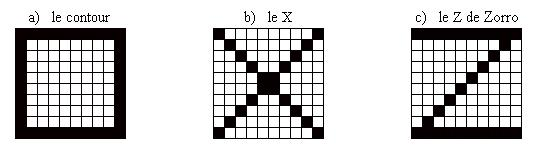
\includegraphics[width=0.9\textwidth]{image/tab2d-ex-oxz}
	\end{center}
\end{Exercice}

\begin{Exercice}{Le tableau de cotes}
	Soit un tableau à $n$ lignes et $m$ colonnes d'entiers où
	une ligne représente les notes sur 20 d'un étudiant et
	les colonnes toutes les notes d'un cours.
	
	Écrire un algorithme recevant ce tableau en paramètre et affichant le
	pourcentage d'étudiants ayant obtenu une moyenne
	supérieure à 50\%.
\end{Exercice}

\begin{Exercice}{Tous positifs}
	\marginicon{java}
	Écrire un module qui reçoit un tableau ($n$ x $m$) d’entiers et qui vérifie
	si tous les nombres qu’il contient sont strictement positifs. Bien sûr,
	on veillera à éviter tout travail inutile; la rencontre d’un nombre
	négatif doit arrêter le module.
\end{Exercice}

\begin{Exercice}{Le carré magique}
	\marginicon{java}
	Un carré magique est un tableau d’entiers carré
	(c'est-à-dire possédant autant de lignes que de
	colonnes) ayant la propriété suivante: si on additionne les éléments
	d'une quelconque de ses lignes, de ses colonnes ou de
	ses deux diagonales, on obtient à chaque fois le même résultat.

	Écrire un module recevant en paramètres le tableau [1 à $n$, 1 à $n$]
	d'entiers carré et renvoyant une valeur booléenne
	indiquant si Carré est un carré magique ou non.
\end{Exercice}

\begin{Exercice}{Le triangle de Pascal}
	Le triangle de Pascal est construit de la façon suivante :

	\begin{liste}
	\item la ligne initiale contient un seul élément de valeur 1 ;
	\item chaque ligne possède un élément de plus que la précédente ;
	\item chaque ligne commence et se termine par 1 ;
	\item 
		pour calculer un nombre d’une autre case du tableau, on additionne le
		nombre situé dans la case située juste au-dessus avec celui dans la
		case à la gauche de la précédente.
	\end{liste}

	Écrire un module qui reçoit en paramètre un entier
	$n$, et qui renvoie un tableau contenant les
	$n+1$ premières lignes du triangle de Pascal
	(indicées de $0$ à $n$).
	
	N.B.: le «~triangle~» sera bien entendu renvoyé dans un tableau carré.
	Quid des cases non occupées ?

	Par exemple, pour $n$ qui vaut 5, on aura le tableau suivant :

	\begin{center}
	\begin{tabular}{|*{6}{>{\centering\arraybackslash}m{0.35cm}|}}
	\hline
	 1 & ~ & ~ & ~ & ~ & ~ \\\hline
	 1 & 1 & ~ & ~ & ~ & ~ \\\hline
	 1 & 2 & 1 & ~ & ~ & ~ \\\hline
	 1 & 3 & 3 & 1 & ~ & ~ \\\hline
	 1 & 4 & 6 & 4 & 1 & ~ \\\hline
	 1 & 5 & 10 & 10 & 5 & 1 \\\hline
	\end{tabular}
	\end{center}
\end{Exercice}

\begin{Exercice}{Le calendrier du mois}
	Écrire un module qui reçoit en paramètres 
	le numéro du premier jour du mois 
	(c-à-d 1 si le mois commence un lundi, 2 si le mois commence un mardi,
	etc.) ainsi que le nombre de jours dans le mois.
	Au départ de ces données, 
	le module remplira avec les dates des jours du mois un tableau
	«~calendrier~» à deux dimensions, 
	dont les colonnes représentent les jours 
	(la première colonne correspondant au lundi) et les lignes les
	semaines. 
	Par exemple, si le mois contient 30 jours et le premier jour
	est un mercredi, le contenu du tableau sera :

	\begin{center}
	\begin{tabular}{|m{0.807cm}|m{0.807cm}|m{0.807cm}|m{0.807cm}|m{0.807cm}|m{0.807cm}|m{0.81100005cm}|}
	\multicolumn{1}{m{0.807cm}}{\centering 
	{L}} &
	\multicolumn{1}{m{0.807cm}}{\centering 
	{M}} &
	\multicolumn{1}{m{0.807cm}}{\centering 
	{M}} &
	\multicolumn{1}{m{0.807cm}}{\centering 
	{{J}}} &
	\multicolumn{1}{m{0.807cm}}{\centering 
	{{V}}} &
	\multicolumn{1}{m{0.807cm}}{\centering 
	{{S}}} &
	\multicolumn{1}{m{0.81100005cm}}{\centering\arraybslash
	 {D}}\\\hline
	~
	 &
	~
	 &
	\raggedleft  {1} &
	\raggedleft  {2} &
	\raggedleft  {3} &
	\raggedleft  {4} &
	\raggedleft\arraybslash 
	{5}\\\hline
	\raggedleft  {6} &
	\raggedleft  {7} &
	\raggedleft  {8} &
	\raggedleft  {9} &
	\raggedleft  {10} &
	\raggedleft  {11} &
	\raggedleft\arraybslash 
	{12}\\\hline
	\raggedleft  {13} &
	\raggedleft  {14} &
	\raggedleft  {15} &
	\raggedleft  {16} &
	\raggedleft  {17} &
	\raggedleft  {18} &
	\raggedleft\arraybslash 
	{19}\\\hline
	\raggedleft  {20} &
	\raggedleft  {21} &
	\raggedleft  {22} &
	\raggedleft  {23} &
	\raggedleft  {24} &
	\raggedleft  {25} &
	\raggedleft\arraybslash 
	{26}\\\hline
	\raggedleft  {27} &
	\raggedleft  {28} &
	\raggedleft  {29} &
	\raggedleft  {30} &
	~
	 &
	~
	 &
	~
	\\\hline
	\end{tabular}
	\end{center}

	\textbf{Réflexions} :

	\begin{liste}
	\item Combien de lignes au maximum doit avoir ce tableau ?
	\item Quid des cases non occupées ?
	\end{liste}
\end{Exercice}

\begin{Exercice}{À vos pinceaux (la suite) !}
	Pour poursuivre l'exercice du pinceau, 
	voici quelques cas plus coriaces.
	
	\begin{center}
	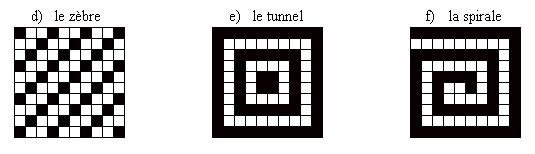
\includegraphics[width=0.9\textwidth]{image/tab2d-ex-zts}
	\end{center}
\end{Exercice}

\begin{Exercice}{Exercices sur la complexité}

	Quelle est la complexité 
	\begin{enumerate}[label=\alph*)]
	\item 
		d’un algorithme de parcours	d'un tableau $n$ x $n$ ?
	\item
		d'un algorithme qui remet à 0 toutes les
		occurrences du maximum d'un tableau $n$ x $n$ ?
	\item 
		de l'algorithme que vous avez écrit pour résoudre les
		exercices du pinceau ?
	\end{enumerate}
\end{Exercice}

\begin{Exercice}{Lignes et colonnes}
	Écrire un module qui reçoit un tableau d’entiers à 2 dimensions en paramètre 
	et qui retourne un booléen indiquant si ce tableau 
	possède 2 lignes ou 2 colonnes identiques.
	
	Dans l’affirmative, 
	ce module renverra également en paramètres les informations suivantes :
	
	\begin{liste}
	\item les indices des lignes ou colonnes identiques
	\item un caractère valant ‘L’ ou ‘C’ selon qu’il s’agit de lignes ou de
	colonnes
	\end{liste}
	
	Dans la négative, les valeurs de ces paramètres seront indéterminées ou
	quelconques, elles ne seront de toute façon pas utilisées par le module
	appelant.
\end{Exercice}

%=================
\chapter{La liste}
%=================

\marginicon{objectif}

Imaginons qu’on désire manipuler par programme une liste de contacts ou
encore une liste de rendez-vous. Cette liste va varier ; sa taille
n’est donc pas fixée. Utiliser un tableau à cet effet n’est pas l’idéal. 
En effet, la taille d’un tableau ne peut plus changer une fois le tableau créé. 
Il faudrait le sur-dimensionner, ce qui n’est pas économe.

Il serait intéressant de disposer d’une structure qui offre toutes les
facilités d’un tableau tout en pouvant «~grandir~» si nécessaire.
Construisons une telle structure de données et appelons-la «~Liste~»
pour rester en phase avec son appellation commune en Java.

Par exemple, considérons une liste de courses.
On pourrait la représenter ainsi :
\begin{enumerate}
\item "fromage"
\item "pain"
\item "salami"
\end{enumerate}

On pourrait ajouter un élément en fin de liste, par exemple de l'eau,
pour obtenir la liste :

\begin{enumerate}
\item "fromage"
\item "pain"
\item "salami"
\item "eau"
\end{enumerate}

On pourrait aussi supprimer un élément de la liste, par exemple le pain,
et obtenir :

\begin{enumerate}
\item "fromage"
\item "salami"
\item "eau"
\end{enumerate}

On pourrait aussi insérer un élément dans la liste, 
par exemple une baguette, 
ce qui décale, de facto, la position des suivants.

\begin{enumerate}
\item "fromage"
\item "salami"
\item "baguette"
\item "eau"
\end{enumerate}

Et encore plein de choses que nous allons détailler.

%========================
\section{La classe Liste}
%=========================

Nous verrons plus loin comment réaliser une classe Liste en pratique 
mais nous pouvons déjà définir le comportement qu’on en attend 
(les méthodes qu’elle doit fournir)

Ce comportement sera indentique quel que soit le type des éléments
de la liste; une liste de chaine et une liste d'entiers
ne se distinguent que par le type de certains paramètres
et valeurs de retour.
Ici, nous indiquons \pseudocode{T} pour indiquer un type quelconque;
vous pouvez le remplacer par ce qui vous convient : entier, chaine, Date\dots.

\begin{Pseudocode}
	\Class{Liste de T}
		\RComment T est un type quelconque
		\Private
			\LComment sera complété plus tard	
		\Public
			\ConstrSign{Liste de T}{}			
				\RComment construit une liste vide
			\MethodSign{get}{pos : entier}{T}
				\RComment donne un élément en position pos
			\MethodSign{set}{pos : entier, valeur : T}{}
				\RComment modifie un élément en position pos
			\MethodSign{taille}{}{entier}
				\RComment donne le nombre actuels d’éléments
			\MethodSign{ajouter}{valeur : T}{}
				\RComment ajoute un élément en fin de liste
			\MethodSign{insérer}{pos : entier, valeur : T}{}
				\RComment insère un élément en position pos
			\MethodSign{supprimer}{}{}
				\RComment supprime le dernier élément
			\MethodSign{supprimerPos}{pos : entier}{}
				\RComment supprime l'élément en position pos
			\MethodSign{supprimer}{valeur : T}{booléen}
				\RComment supprime l'élément de valeur donnée
			\MethodSign{vider}{}{}
				\RComment vide la liste
			\MethodSign{estVide}{}{booléen}
				\RComment la liste est-elle vide ?
			\MethodSign{existe}{valeur \In : T, pos \Out : entier}{booléen}
				\RComment recherche un élément
		\EndClass
\end{Pseudocode}

\bigskip

Quelques précisions s’imposent :
\begin{liste}
	%\item 
		%Comme les tableaux, les listes peuvent contenir des éléments de
		%n’importe quel type tout en restant uniforme au sein d’une même liste
		%(on pourra manipuler une liste d’entiers, une liste de contacts\dots\ 
		%mais pas mélanger). Il serait rédhibitoire de devoir définir une Liste
		%pour chaque type d’éléments. On utilise dès lors la possibilité en OO
		%d’écrire un code \textbf{générique}\footnote{\ on parle aussi de
		%«~template~».}. Le «~T~» dans la définition de la classe indique le
		%type des éléments qui sera spécifié lors de l’utilisation de la classe.
		%On écrira par exemple «~\pseudocode{Liste d’entiers}~» pour
		%utiliser une liste d’entiers.
	\item 
		Les méthodes «\pseudocode{~get~}» et «\pseudocode{~set~}»
		permettent de connaitre ou modifier un élément de la liste. On
		considère, au cours d'algorithmique, que le premier élément de 
		la liste est en position 1.
	\item 
		«\pseudocode{~ajouter~}» ajoute un élément en fin de liste (elle
		grandit donc d’une unité)
	\item 
		«\pseudocode{~insérer~}» insère un élément à une position donnée
		(entre 1 et taille+1). L’élément qui s’y trouvait est décalé
		d'une position ainsi que tous les éléments suivants.
	\item 
		La méthode «\pseudocode{~supprimerPos~}»
		supprime un élément d'une position donnée en
		décalant les éléments suivants. On pourrait imaginer une technique plus
		rapide consistant à placer le dernier élément à la place de l’élément
		supprimé mais ce faisant on changerait l’ordre relatif des éléments ce
		qui va à l’encontre de l’idée intuitive qu’on se fait d’une liste.
		Cette amélioration pourrait plutôt s’envisager dans une structure de
		type \textbf{ensemble} pour lequel il n’y a pas d’ordre relatif entre
		les éléments.
	\item 
		La version de «\pseudocode{~supprimer~}» avec une valeur en
		paramètre enlève un élément de valeur donnée. Elle retourne un booléen
		indiquant si la suppression a pu se faire ou pas (ce qui sera le cas si
		la valeur n’est pas présente dans la liste). Si la valeur existe en
		plusieurs exemplaires, on prendra la convention arbitraire que
		la méthode n’en supprime que la première	occurrence.
	\item 
		La méthode «\pseudocode{~existe~}» permet de savoir si un élément
		donné existe dans la liste. 
		\begin{liste}
			\item 
				si c’est le cas, elle précise aussi sa position dans le paramètre sortant 
				\pseudocode{pos}
			\item 
				si l’élément n’existe pas, ce paramètre est	indéterminé 
			\item 
				si l’élément est présent en plusieurs exemplaires, la méthode donne la
				position de la première occurrence.
		\end{liste}
	\item 
		En pratique, il serait intéressant de chercher un élément à partir d’une
		partie de l’information qu’elle contient mais c’est difficile à
		exprimer de façon générique c'est-à-dire lorsque le
		type n'est pas connu à priori.
\end{liste}

{\sffamily\bfseries\scshape
Exemple : manipulations de base}

Soit l'algorithme suivant :

\begin{Pseudocode}
	\Module{ex1}{}{}
		\Decl l : Liste d'entiers
		\Let l \Gets \K{nouvelle} Liste d'entiers()
		\Stmt l.ajouter(42)
		\Stmt l.ajouter(54)
		\Stmt l.set(2,44)
		\Stmt l.insérer(2,43)
		\Stmt l.supprimerPos(3)
		\Stmt l.supprimer(42)
		\Stmt l.vider
	\EndModule
\end{Pseudocode}

Après sa création, la liste est vide.
Ensuite, elle passe par les états suivants :

\begin{minipage}[t]{2cm}
\begin{enumerate}
\item 42
\end{enumerate}
\end{minipage}
\begin{minipage}[t]{2cm}
\begin{enumerate}
\item 42
\item 54
\end{enumerate}
\end{minipage}
\begin{minipage}[t]{2cm}
\begin{enumerate}
\item 42
\item 44
\end{enumerate}
\end{minipage}
\begin{minipage}[t]{2cm}
\begin{enumerate}
\item 42
\item 43
\item 44
\end{enumerate}
\end{minipage}
\begin{minipage}[t]{2cm}
\begin{enumerate}
\item 42
\item 43
\end{enumerate}
\end{minipage}
\begin{minipage}[t]{2cm}
\begin{enumerate}
\item 43
\end{enumerate}
\end{minipage}

Enfin, le dernier appel la vide complètement

\bigskip
{\sffamily\bfseries\scshape
Exemple : recherche du minimum}

Dans le chapitre sur les tableaux, vous avez fait un exercice consistant
à afficher tous les indices où se trouve le minimum d’un tableau.
Reprenons-le et modifions-le afin qu’il retourne la liste des indices
où se trouvent les différentes occurrences du minimum. On pourrait
l’écrire ainsi :

\begin{Pseudocode}
	\Module{indicesMinimum}{tab : tableau [1 à n] d'entiers}{Liste d'entiers}
		\Decl i, min : entier
		\Decl indicesMin : Liste d'entiers
		\Let min \Gets tab[1]
		\Let indicesMin \Gets \K{nouvelle} Liste d'entiers()
		\Stmt indicesMin.ajouter( 1 )
		\For{i \K{de} 2 \K{à} n}
			\Switch{} 
				\Case{tab[i] = min}
					\Stmt indicesMin.ajouter( i )
				\Case{tab[i] < min}
					\Stmt indicesMin.vider() 
					\Stmt indicesMin.ajouter( i )
					\Let min \Gets tab[i]
				\Case{tab[i] > min}
					\LComment rien à faire dans ce cas	
			\EndSwitch
		\EndFor
		\Return indicesMin
	\EndModule
\end{Pseudocode}

\clearpage
%===================================
\section{Comment implémenter l’état}
%===================================

Cette liste est bien utile mais comment la réaliser en pratique ?
Comment représenter une liste variable d’éléments ? Pour
l'instant, la seule structure qui peut accueillir
plusieurs éléments de même type est le tableau. Nous allons donc
prendre comme attribut principal de la liste, un tableau que nous
appellerons \pseudocode{éléments}. Comment, dès lors, contourner
le problème de la limitation de la taille de ce tableau ?

Repartons donc de la notion de tableau et tentons de comprendre sa
limitation. Lors de sa création, un tableau se voit attribuer un espace
bien précis et contigu en mémoire. Il se peut très bien que
l'espace «~juste après~» soit occupé par une autre
variable ce qui l'empêche de grandir. La parade est
claire : si un \ tableau s’avère trop petit lors de son utilisation, il
suffit d’en créer un autre plus grand ailleurs en mémoire et d’y
recopier tous les éléments du premier. Évidemment, cette opération est
coûteuse en temps et on cherchera à l’effectuer le moins souvent
possible.

\textbf{Quelle taille donner au nouveau tableau} ? L’idée qui vient
immédiatement est d’augmenter la taille d’une unité afin d’accueillir
le nouvel élément mais cette approche implique de fréquents
agrandissements. Il est plus efficace d’augmenter la taille
proportionnellement, par exemple en la multipliant par un facteur 2.

\begin{center}
\begin{tabular}{|m{0.259cm}|m{0.259cm}|m{0.259cm}|m{0.087999985cm}m{0.46000004cm}m{0.087999985cm}|m{0.25300002cm}|m{0.259cm}|m{0.259cm}|m{0.15299998cm}|m{0.15299998cm}|m{0.17cm}|}
\hhline{---~~~------}
 1 &
 5 &
 7 &
~
 &
 ${\Rightarrow}$ &
~
 &
 1 &
 5 &
 7 &
 . &
 . &
 .\\\hhline{---~~~------}
\end{tabular}
\end{center}


\textbf{Taille logique et taille physique}. À tout moment, le tableau
aura une et une seule taille même si celle-ci pourra changer au cours
du temps. Puisqu’on multipliera la taille du tableau par 2 pour des
raisons d’efficacité, il y aura toutefois une différence entre la
\textbf{taille physique} d’un tableau et sa \textbf{taille logique}. La
taille physique est le nombre de cases réservées pour le tableau alors
que la taille logique est le nombre de cases effectivement occupées.
Dans ce qui suit, on s'arrangera pour que les cases
occupées soient groupées à gauche du tableau (il n'y a
pas de trou). Pour l’utilisateur, seule la taille logique a un sens (on
lui cache les détails d’implémentation).

\textbf{Exemple} : pour le tableau suivant, la taille logique est de 6
(c’est cette taille qui a du sens pour l’utilisateur de la liste) et la
taille physique est de 8.

\begin{center}
\begin{tabular}{|m{0.506cm}|m{0.506cm}|m{0.506cm}|m{0.506cm}|m{0.506cm}|m{0.506cm}|m{0.506cm}|m{0.523cm}|}
\hline
 2 &
 5 &
 4 &
 8 &
 3 &
 12 &
\centering  . &
\centering\arraybslash  .\\\hline
\end{tabular}
\end{center}

Quand il faut insérer un élément (en position valide) ou en ajouter un
en fin de liste, deux cas se présentent :

\begin{liste}
	\item 
		si la taille logique est plus petite que la taille physique, il suffit
		d’ajouter l’élément dans le tableau et d’adapter la taille logique.
	\item 
		si la taille logique est égale à la taille physique, il faut
		procéder à un agrandissement du tableau.
\end{liste}

\textbf{Les tableaux dynamiques}. 
En \emph{DEV$_1$},
nous n'avons vu que des tableaux
qu'on appellera \emph{statiques},
qui sont créés lors de leur déclaration.
Ici, nous avons besoin de tableaux 
qu'on appellera \emph{dynamiques},
créés dans le code
(comme le sont les tableaux en Java).

Introduisons une notation.
Un tableau dynamique sera déclaré puis créé ainsi :

	\begin{Pseudocode}
		\Decl tab~: \K{tableau} de chaines
		\Let tab \Gets \K{nouveau} \K{tableau} [1 à n] de chaines \RComment n doit avoir une valeur
	\end{Pseudocode}

\textbf{Implémentation}.
Présentons les attributs nécessaires et l'algorithme
d’agrandissement du tableau.

\begin{Pseudocode}
	\Class{Liste de T}
		\Private
			\Decl éléments : \K{tableau} de T
			\Decl tailleLogique : entier
			\Decl taillePhysique : entier
		\Private
			\Method {agrandir}{}{}
				\Decl i : entier
				\Decl nouveauTab : \K{tableau} de T
				\Let taillePhysique \Gets taillePhysique * 2
				\Let nouveauTab \Gets \K{nouveau} \K{tableau} [ 1 à taillePhysique ] de T
				\For{i \K{de} 1 \K{à} tailleLogique}
					\Let nouveauTab[ i ] \Gets éléments[ i ]
				\EndFor
				\Let éléments \Gets nouveauTab
			\EndMethod
		\EndClass
	\end{Pseudocode}

\bigskip

\textbf{Réduction du tableau}. Tout comme on agrandit le tableau si
nécessaire, on pourrait le réduire lorsque des suppressions d’éléments
le rendent sous-utilisé (par exemple lorsque la taille logique devient
inférieure au tiers de la taille physique). 
Nous n'aborderons pas cette problématique cette année.


%=======================================
\section{Implémentation du comportement}
%=======================================

Nous avons à présent toutes les cartes en main pour écrire les méthodes
publiques de la classe.

\begin{Pseudocode}
	\Constr{Liste de T}{}
		\Let tailleLogique \Gets 0
		\RComment la liste est vide au départ
		\Let taillePhysique \Gets 32
		\RComment une bonne valeur pour commencer
		\Let éléments \Gets \K{nouveau} \K{tableau} [ 1 à taillePhysique ] de T
	\EndConstr
\end{Pseudocode}

\begin{Pseudocode}
	\Method{get}{pos : entier}{T}
		\If{ pos < 1 OU pos > tailleLogique}
			\Error "position invalide"
		\EndIf
		\Return éléments[ pos ]
	\EndMethod
\end{Pseudocode}

\begin{Pseudocode}
	\Method{set}{pos : entier, valeur : T}{}
		\If{ pos < 1 OU pos > tailleLogique}
			\Error "position invalide"
		\EndIf
		\Let éléments[ pos ] \Gets valeur
	\EndMethod
\end{Pseudocode}

\begin{Pseudocode}
	\Method{taille}{}{entier}
		\Return tailleLogique
		\RComment et pas la taille physique !
	\EndMethod
\end{Pseudocode}

\begin{Pseudocode}
	\Method{ajouter}{valeur : T}{}
		\If{tailleLogique = taillePhysique}
			\Stmt agrandir()
			\RComment méthode privée détaillée supra
		\EndIf
		\Let tailleLogique \Gets tailleLogique + 1
		\Let éléments[ tailleLogique ] \Gets valeur
	\EndMethod
\end{Pseudocode}

\begin{Pseudocode}
	\Method{insérer}{pos : entier, valeur : T}{}
		\If{ pos < 1 OU pos > tailleLogique+1}
			\Error "position invalide"
		\EndIf
		\If{tailleLogique = taillePhysique}
			\Stmt agrandir()
		\EndIf
		\Stmt décalerDroite( pos )
		\RComment voir ci-dessous
		\Let tailleLogique \Gets tailleLogique + 1
		\Let éléments[ pos ] \Gets valeur
	\EndMethod
\end{Pseudocode}

\begin{Pseudocode}
	\Method{supprimer}{}{}
		\LComment supprime le dernier élément
		\If{tailleLogique = 0}
			\Error "liste vide"
		\EndIf
		\Let tailleLogique \Gets tailleLogique - 1
	\EndMethod
\end{Pseudocode}

\begin{Pseudocode}
	\Method{supprimerPos}{pos : entier}{}
		\If{ pos < 1 OU pos > tailleLogique}
			\Error "position invalide"
		\EndIf
		\Stmt décalerGauche( pos + 1 )
		\RComment voir méthode ci-dessous
		\Let tailleLogique\Gets tailleLogique - 1
	\EndMethod
\end{Pseudocode}

\begin{Pseudocode}
	\Method{supprimer}{valeur: T}{booléen}
		\Decl estPrésent : booléen
		\Decl pos : entier
		\Let estPrésent \Gets existe(valeur, pos)
		\If{estPrésent}
			\Stmt supprimer( pos )
		\EndIf
		\Return estPrésent
	\EndMethod
\end{Pseudocode}

\begin{Pseudocode}
	\Method{vider}{}{}
		\Let tailleLogique \Gets 0 
		\RComment Les éléments ne sont pas effacés mais sont ignorés
	\EndMethod
\end{Pseudocode}

\begin{Pseudocode}
	\Method{estVide}{}{booléen}
		\Return tailleLogique = 0
	\EndMethod
\end{Pseudocode}

\begin{Pseudocode}
	\Method{existe}{valeur\In : T, pos\Out : entier}{booléen}
		\Let pos \Gets 1
		\LComment Rq : le ET ci-dessous est une évaluation 
		court-circuitée (cf. le cours d'Algo en DEV1)
		\While{ pos {${\leq}$} tailleLogique ET éléments[ pos ] {${\neq}$} valeur}
			\Let pos \Gets pos + 1
		\EndWhile
		\Return pos {${\leq}$} tailleLogique
	\EndMethod
\end{Pseudocode}

\begin{Pseudocode}
	\LComment Ces méthodes-ci sont privées
	\bigskip

	\Method{décalerDroite}{début : entier}{}
		\LComment Décale tous les éléments d'une position vers
		la droite à partir de début
		\Decl i : entier
		\For{i \K{de} tailleLogique \K{à} début \K{par} –1}
			\Let éléments[ i + 1 ] \Gets éléments[ i ]
		\EndFor
	\EndMethod

	\bigskip
	
	\Method {décalerGauche}{début : entier}{}
		\LComment Décale toutes les éléments d'une position vers
		la gauche à partir de début ; 
		\LComment ce paramètre vaut toujours au moins 2.
		\Decl i : entier
		\For{i \K{de} début \K{à} tailleLogique}
			\Let éléments[ i - 1 ] \Gets éléments[ i ]
		\EndFor
	\EndMethod
\end{Pseudocode}

\bigskip

\marginicon{attention}
\textbf{La recherche se fait sur un élément complet.}

Prenons comme exemple une liste de contacts.
Lors d'une recherche, on doit fournir
\textbf{tout} le contact à
rechercher. Il s'agit juste de savoir
s'il est présent et où. Une autre méthode intéressante
serait de retrouver un contact à partir d'une partie
de l'information, par exemple son nom. Cette méthode
est fort proche de notre méthode de recherche mais il serait très
difficile de l'écrire génériquement. On vous demandera
d'écrire explicitement une telle méthode de recherche
en cas de besoin.


%====================================
\section{Et sans tableau dynamique ?}
%=====================================

Certains langages (c’est le cas de Cobol) ne permettent pas de créer
dynamiquement un nouveau tableau. Il vous faudra travailler avec un
tableau classique en le créant suffisamment grand.


Les algorithmes d’ajout/suppression/recherche vus pour la liste peuvent
être appliqués tels quels à un tableau statique à une modification près
: lors d’un ajout dans un tableau plein, on ne peut pas l’agrandir; il
faut générer une erreur.


%==================
\section{Exercices}
%===================

\begin{Exercice}{Liste des premiers entiers}
	Écrire un module qui reçoit un entier $n$ en paramètre et retourne la
	liste contenant les entiers de 1 à $n$ dans l'ordre
	décroissant. On peut supposer que $n$ est positif.
\end{Exercice}
	
\begin{Exercice}{Somme d'une liste}
	\marginicon{java}
	Écrire un module qui calcule la somme des éléments d’une liste
	d’entiers.
\end{Exercice}

\begin{Exercice}{Les extrêmes}
		\marginicon{java}
		Écrire un module qui supprime le minimum et le maximum des éléments
		d’une liste d’entiers. On peut supposer que le maximum et le minimum
		sont uniques.
\end{Exercice}

\begin{Exercice}{Anniversaires}
		\marginicon{java}
		Écrire un module qui reçoit une liste de Personne (nom + prénom + date
		de naissance ; cf. exercice dans le chapitre OO) et retourne la liste
		de ceux qui sont nés durant un mois passé en paramètre (donné sous la 
		forme d'un entier entre 1	et 12).
\end{Exercice}
	
\begin{Exercice}{Concaténation de deux listes}
		\marginicon{java}
		Écrire un module qui reçoit 2 listes et ajoute
		à la suite de la première les éléments de la seconde; la seconde liste
		n'est pas modifiée par cette opération.
\end{Exercice}

\begin{Exercice}{Fusion de deux listes}
		\marginicon{java}
		Soit deux listes \textbf{ordonnées}
		d'entiers (redondances possibles). Écrire un module
		qui les fusionne. Le résultat est une liste encore ordonnée contenant
		tous les entiers des deux listes de départ (qu'on
		laisse inchangées).

		Exemple : Si les 2 listes sont (1, 3, 7, 7) et (3, 9), 
		le résultat est (1, 3, 3, 7, 7, 9).
\end{Exercice}

\begin{Exercice}{Le nettoyage}
	Écrire un module qui reçoit une liste de chaines en paramètre et
	supprime de cette liste tous les éléments de valeur donnée en
	paramètre. L'algorithme retournera le nombre de
	suppressions effectuées.
\end{Exercice}
	
\begin{Exercice}{Éliminer les doublons d'une liste}
		Soit une liste \textbf{ordonnée} 
		d'entiers avec de possibles redondances. Écrire un
		module qui enlève les redondances de la liste.
				
		Exemple : Si la liste est (1, 3, 3, 7, 8, 8, 8),
		le résultat est (1, 3, 7, 8).

		\begin{enumerate}[label=\alph*)]
			\item 
				Faites l'exercice en créant une \textbf{nouvelle
				liste} (la liste de départ reste inchangée)
			\item 
				Refaites l'exercice en \textbf{modifiant}
				la liste de départ (pas de nouvelle liste)
		\end{enumerate}
\end{Exercice}

%\begin{Exercice}{Perfectionnement de la classe Liste}
	%Dans l’implémentation de la liste, nous avons écrit 
	%une méthode privée \pseudocode{agrandir} qui remplace le tableau 
	%\pseudocode{éléments} par un autre tableau deux fois plus grand. 
	%On demande à présent d’implémenter dans la classe 
	%une méthode \pseudocode{rétrécir}, qui consistera à diviser la 
	%taille physique du tableau par 2 lorsque la taille 
	%logique devient inférieure au tiers de la taille physique.
	%Adapter également le code des méthodes qui sont concernées 
	%par ce rétrécissement du tableau éléments.

%\end{Exercice}

%\begin{Exercice}{Une classe texte}
	%Un texte est composé de mots et de caractères de ponctuation. 
	%Ils sont séparés par des espaces (caractères «~blanc~») dont 
	%nous ne tenons pas compte ici. Dans notre implémentation, nous 
	%représenterons les mots par des chaines et les caractères de ponctuation 
	%(‘.’, ‘?’, ‘!’, ‘~:’, ‘;’,~etc.) par des chaines d’un seul caractère. 
	%Un texte peut alors être vu comme une Liste <chaines>. 
	%Exemple~: le texte <<Qu’il est bon d’être à l’ESI~!>>
	%sera représenté par une liste contenant les 13 éléments suivants~:
	%\begin{center}
	%\begin{tabular}{|m{8cm}|}
		%\hline
		%Qu \\
		%’	\\
		%il \\
		%est \\
		%bon \\
		%d \\
		%’ \\
		%être \\
		%à \\
		%l \\
		%’ \\
		%ESI \\
		%! \\\hline
	%\end{tabular}
	%\end{center}
	
	%Nous allons définir une classe Texte dont le seul attribut privé sera~: 
	%\pseudocode{listeTxt~: Liste <chaines>}
	%On demande d’écrire~:
	%\begin{enumerate}
	%\item
		%un constructeur sans paramètre créant un texte vide
	%\item
		%un constructeur recevant en paramètre un tableau de chaines 
		%(possédant $n$ éléments) et qui initialise le texte avec 
		%le contenu du tableau
	%\item
		%une méthode 
		%\pseudocode{taille()} qui retourne le nombre de mots du texte 
		%(les caractères de ponctuation ne sont pas comptés par cette méthode~; 
		%ainsi, la taille du texte de l’exemple ci-dessus est 9)
	%\item
		%une méthode 
		%\pseudocode{extrait(départ, nombre~: entier) $\rightarrow$ Texte} 
		%qui retourne la portion de texte débutant à l’indice départ 
		%de la liste et possédant le nombre d’éléments spécifié par 
		%le paramètre nombre (mots et caractères de ponctuation confondus). 
		%Par exemple, extrait(5, 4) appliqué au texte ci-dessus renverrait 
		%le texte <<bon d’être>>
	%\item
		%une méthode 
		%\pseudocode{identique(autreTexte~: Texte) $\rightarrow$ booléen} 
		%qui indique si 2 textes sont identiques au caractère de ponctuation près
	%\item
		%une méthode 
		%\pseudocode{quasiIdentique(autreTexte~: Texte) $\rightarrow$ booléen} 
		%qui indique si les mots des 2 textes sont les mêmes, des différences 
		%pouvant être admises au niveau de la ponctuation. Par exemple, les textes~:
		
		%<<Il m’a dit, en me regardant dans les yeux, que j’étais stupide.>>
		
		%et
		
		%<<Il m’a dit en me regardant dans les yeux que j’étais… «~stupide~»~!>>
		
		%sont quasi identiques, mais pas identiques.
	%\end{enumerate}
		%Détaillez le code de cette classe. Vous pouvez utiliser (sans le détailler) le module
		%\pseudocode{estPonctuation(ch~: chaine) $\rightarrow$ booléen}
		%qui indique si une chaine est un caractère de ponctuation.
			
%\end{Exercice}

	
%\begin{Exercice}{La liste ordonnée}
		%Une recherche dans une liste implique un parcours complet de la liste en
		%cas de recherche infructueuse. La recherche pourrait être plus rapide
		%si la liste était ordonnée (en utilisant la recherche dichotomique). La
		%contrainte principale est qu'il faudra maintenir le
		%caractère ordonné de la liste (notamment en cas
		%d'ajout). Écrivez les modules suivants, de façon à ce
		%que la liste reste ordonnée.

		%\begin{Pseudocode}
			%\ModuleSign{ajouterOrdonné}{liste : Liste de T, valeur : T}{}
			%\ModuleSign{enleverOrdonné}{liste : Liste de T, valeur : T}{booléen}
			%\LComment retourne faux si valeur pas présente. 
			%\LComment Si la valeur est présente en plusieurs exemplaire, en enlève une.
			%\ModuleSign{existeOrdonné}{liste\In : Liste de T, valeur\In : T, pos\Out: entier}{booléen}
			%\LComment si la valeur n'est pas trouvée, pos donne la position où elle aurait dû être.
		%\end{Pseudocode}

%\end{Exercice}

%\begin{Exercice}{Trier des mots}
		%Écrivez un algorithme qui lit une série de mots (se terminant par une
		%chaine vide) sans aucun ordre et les affiche dans l’ordre alphabétique.
		%Vous pouvez utiliser les modules écrits lors de
		%l'exercice précédent.
		
%\end{Exercice}

%\begin{Exercice}{Éviter les doublons}
		%Modifiez l’exemple ci-dessus pour que deux mots identiques ne soient
		%introduits qu’une seule fois dans la liste.
%\end{Exercice}

%\begin{Exercice}{L'ensemble}
		%La notion d’ensemble fini est une notion qui vous est déjà 
		%familière pour l’avoir rencontrée dans plusieurs cours. Nous rappelons
		%certaines de ses propriétés et opérations. 
				
		%Étant donnés deux ensembles
		%finis \textbf{S} et \textbf{T} ainsi qu’un élément \textbf{x} :

		%\begin{liste}
		%\item 
			%\textbf{x} {${\in}$} \textbf{S} signifie que l’élément \textbf{x}
			%est un élément de l’ensemble \textbf{S}.
		%\item 
			%L’ensemble vide, noté \textbf{${\emptyset}$} 
			%est l’ensemble qui n’a pas d’élément 
			%(\textbf{x} {${\in}$} \textbf{${\emptyset}$} 
			%est faux quel que soit \textbf{x} ).
		%\item 
			%L’ordre des éléments dans un ensemble n’a
			%aucune signification, l’ensemble \{1,2\} est
			%identique à \{2,1\}.
		%\item 
			%Un élément \textbf{x} ne peut
			%pas être plus d’une fois élément d’un même ensemble 
			%(pas de répétition).
		%\item 
			%L’union \textbf{S ${\cup}$ T} 
			%est l’ensemble contenant les éléments qui sont dans 
			%\textbf{S} ou (non exclusif) dans \textbf{T}.
		%\item 
			%L’intersection \textbf{S ${\cap}$ T} 
			%est l’ensemble des éléments qui sont à la fois 
			%dans \textbf{S} et dans \textbf{T}.
		%\item 
			%La différence \textbf{S {\textbackslash} T} 
			%est l’ensemble des éléments qui sont 
			%dans \textbf{S} mais pas dans \textbf{T}.
		%\end{liste}
		
		%Créez la classe \pseudocode{Ensemble}
		%décrite ci-dessous.
		
		%\begin{Pseudocode}
			%\Class{Ensemble <T>}{} 
			%\RComment T est le type des éléments de l'ensemble
			
				%\Public
				%\ConstrSign{Ensemble <T>}{} 
				%\RComment construit un ensemble vide
				%\MethodSign{ajouter}{élt : T}{}
				%\RComment ajoute l'élément à l'ensemble
				%\MethodSign{enlever}{élt : T}{})
				%\RComment enlève un élément de l'ensemble
				%\MethodSign{contient}{élt : T}{booléen}
				%\RComment dit si l'élément est présent
				%\MethodSign{estVide}{}{booléen}
				%\RComment dit si l'ensemble est vide
				%\MethodSign{taille}{}{entier}
				%\RComment donne la taille de l'ensemble
				%\MethodSign{union}{autreEnsemble : Ensemble <T>}{Ensemble <T>}
				%\MethodSign{intersection}{autreEnsemble : Ensemble <T>}{Ensemble <T>}
				%\MethodSign{moins}{autreEnsemble : Ensemble <T>}{Ensemble <T>}
				%\MethodSign{listeÉléments}{}{Liste <T>}
				%\RComment conversion en liste
			%\EndClass
		%\end{Pseudocode}
		
	%\bigskip

	%Quelques remarques :

	%\begin{liste}
		%\item 
			%La méthode d'ajout (resp. de suppression) n'a
			%pas d'effet si l'élément est déjà
			%(resp. n'est pas) dans l'ensemble.
		%\item 
			%Les méthodes \pseudocode{union()}, 
			%\pseudocode{intersection()} et 
			%\pseudocode{moins()} retournent un troisième ensemble, 
			%résultat des 2 premiers sans toucher
			%à ces 2 ensembles. On aurait pu envisager des méthodes modifiant
			%l'ensemble sur lequel on les appelle.
		%\item 
			%La méthode \pseudocode{listeÉlément()}
			%est nécessaire si on veut parcourir les éléments de
			%l'ensemble (par exemple pour les afficher).
	%\end{liste}
%\end{Exercice}

%\begin{Exercice}{Autres opérations ensemblistes}
	%Nous avons défini des opérations ensemblistes ne touchant pas aux
	%ensembles de départ. Que deviennent-elles si on considère
	%qu'elles \textbf{modifient}
	%l'ensemble sur lequel elles sont appliquées ?
%\end{Exercice}

\begin{Exercice}{Rendez-vous}
	Soit la structure «\pseudocode{~RendezVous~}» composée d’une date
	et d’un motif de rencontre. Écrire un module qui reçoit une liste de
	rendez-vous et la met à jour en supprimant tous ceux qui sont désormais
	passés. 
\end{Exercice}

%===================================
\chapter{Représentation des données%
\index{Representation des données@Représentation des données}}
%====================================

Nous voici arrivés au terme de ce cours d'algorithmique. 
Ce chapitre apporte une synthèse des différentes notions vues 
tout au long de vos cours d'algorithmiques de 1\iere\ année 
et propose quelques pistes de réflexion 
quant au choix d’une bonne représentation des données 
qui se pose lors de la résolution de problèmes de programmation avancés.

Pour la plupart de ces exercices,
la difficulté tient en partie dans le bon choix d’une représentation des données 
et de la démarche algorithmique la plus adéquate à mettre en œuvre pour agir sur ces
données en vue d’obtenir le résultat escompté. Noter que l’efficacité
d’un algorithme est lié étroitement au choix de la représentation.

%======================================
\section{Se poser les bonnes questions}
%=======================================

Revenons à la case départ : nous avons commencé ce cours en situant les
notions de \textbf{problème} et de \textbf{résolution}. Nous avons vu
qu’un problème bien spécifié s’inscrit dans le schéma :

\cadre{
étant donné [les données] on demande [l’objectif]
}

Une fois le problème correctement posé, on peut partir à la recherche
d’une \textbf{méthode de résolution}, c’est-à-dire d’un algorithme en
ce qui concerne les problèmes à résoudre par les moyens informatiques.

Tout au long de l’année, nous avons vu divers modèles et techniques
algorithmiques adaptées à des structures particulières (les nombres,
les chaines, les tableaux, les variables structurées, les objets, les
listes\dots). La plupart des exercices portaient directement
sur ces structures (par ex. calculer la somme des nombres d’un tableau,
extraire une sous-liste à partir
d’une liste donnée). Ces exercices d’entrainement et de formation
quelque peu théoriques constituent en fait des démarches algorithmiques
de base qui trouvent toutes une place dans des problèmes plus
complexes.

Mais la plupart des problèmes issus des situations de la vie courante
auxquels se confronte le programmeur s’expriment généralement de
manière plus floue : par ex. dresser la comptabilité des dépenses
mensuelle d’une firme, faire un tableau récapitulatif du résultat des
élections par cantons électoraux, faire une version informatique d’un
jeu télévisé… Les exemples sont infinis !


C’est dans le cadre de ce genre de problème plus complexe que se pose le
problème de la \textbf{représentation de données}. Une fois le problème
bien spécifié (par les données et l’objectif) apparaissent
naturellement les questions suivantes : quelles données du problème
sont réellement utiles à sa résolution ?~(Il est fréquent que l’énoncé
d’un problème contienne des données superflues ou inutiles). Y a-t-il
des données plus importantes que d’autres ? (données principales ou
secondaire). Les données doivent-elles être consultées plusieurs fois ?
Quelles données faut-il conserver en mémoire ? Sous quelle forme ?
Faut-il utiliser un tableau ? Une liste ? Faut-il créer une nouvelle
classe ? Les données doivent-elles être classées suivant un critère
précis ? Ou la présentation brute des données suffit-elle pour
solutionner le problème posé ?

Les réponses ne sont pas directes, et les différents outils qui sont à
notre disposition peuvent être ou ne pas être utilisés. Il n’y a pas de
règles précises pour répondre à ces questions, c’est le flair et le
savoir-faire développés patiemment par le programmeur au fil de ses
expériences et de son apprentissage qui le guideront vers la solution
la plus efficace. Parfois plusieurs solutions peuvent fonctionner sans
pouvoir départager la meilleure d’entre-elles.

Ce type de questionnement est peut-être l’aspect le plus délicat et le
plus difficile de l’activité de programmation, car d’une réponse
appropriée dépendra toute l’efficacité du code développé. Un mauvais
choix de représentation des données peut mener à un code lourd et
maladroit. Nous donnons dans ce qui suit quelques indices et pistes de
réflexion, qui seront consolidées par l’expérience acquise lors des
laboratoires de langages informatiques ainsi que par les techniques de
modélisation vues au cours d’analyse.


%==================================
\section{Les structures de données%
\index{Structures de donnees@Structures de données}}
%==================================

Rappelons brièvement les différentes structures étudiées dans ce cours
\index{Structures a connaitre@Structures à connaitre} :

\begin{liste}
	\item 
		les \textbf{données «~simples~»} (variables isolées : entiers, réels,
		chaines, caractères, booléens)
	\item 
		les \textbf{variables structurées}, qui regroupent en une seule entité
		une collection de variables simples
	\item 
		le \textbf{tableau}, qui contient un nombre déterminé de variables de
		même types, accessibles via un indice ou plusieurs pour les tableaux
		multidimensionnels
	\item 
		les \textbf{objets}, qui combinent en un tout une série d’attributs et
		des méthodes agissant sur ces attributs
	\item 
		la \textbf{liste}, qui peut contenir un nombre indéfini d’éléments de
		même type
	%\item 
		%le \textbf{fichier séquentiel}, qui est un support physique permettant
		%le stockage «~à long terme~» de données
\end{liste}

D’autres structures particulières s’ajouteront dans le cours de
2\textsuperscript{e} année : les listes chainées, les piles, les
files, les arbres et les graphes.

Chacune de ces structures possède ses spécificités propres quant à la
façon d’accéder aux valeurs, de les parcourir, de les modifier,
d’ajouter ou de supprimer des éléments à la collection. 

%%========================================
%\section{Quelques conseils pour terminer}
%%========================================

%Nous vous conseillons de relire le paragraphe 4.7 du
%cours d'algorithmique de DEV1 intitulé
%:~«~\textit{qu’est-ce qu’un algorithme de qualité ?}~». 
%Après une année d’apprentissage, 
%vous comprendrez certainement sous un nouvel éclairage
%les termes de validité, d’extensibilité, de réutilisabilité, de
%lisibilité et d’efficience.

%Outre ces grands principes de base, ajoutons ici quelques conseils en
%vrac qui pourraient vous être utiles :

%\begin{liste}
	%\item 
		%\textbf{parcours des données} : en général on évite de parcourir
		%plusieurs fois le contenu d’un ensemble de données (surtout s’il s’agit
		%d’un fichier) sauf s’il n’y a pas d’autre solution.
	%\item 
		%\textbf{duplication des données} : on évite également de créer un
		%duplicata sous quelque forme que ce soit d’une grande structure de
		%données. Par exemple, s’il faut trier les données d’un fichier, il est
		%évident qu’il faut stocker l’entièreté des données en mémoire~pour
		%pouvoir effectuer les comparaisons ; par contre, c’est inutile si le
		%problème est d’extraire le maximum de ces données ou de les compter
	%\item 
		%\textbf{les booléens} : rappelons l’utilité des variables booléennes !
		%L’expérience montre que les étudiants négligent souvent leur
		%utilisation. Elles permettent de décrire de façon élégante l’état de
		%différentes situations, d’exprimer de façon concise des conditions…
	%\item 
		%\textbf{choix des boucles} : relisez attentivement le paragraphe 7.2 sur
		%le choix des boucles. Dans un processus itératif, il est impératif de
		%le quitter dès qu’une réponse est connue, plutôt que de parcourir
		%inutilement jusqu’au bout un ensemble de données. Le bon suivi de ce
		%principe intervient de façon primordiale dans l’efficacité d’un
		%algorithme ! 
%\end{liste}

\clearpage
%==================
\section{Exercices}
%==================

\begin{Exercice}{Le lièvre et la tortue}

	\emph{lu sur le net} :
	{\footnotesize \url{http://mathemathieu.free.fr/2b/doc/pb_algo/problemes_et_algorithmique.pdf}}
	
	Le lièvre est plus rapide que la tortue.
	Pour donner plus de chance à la tortue de gagner une course de 5 km, 
	on adopte la règle de jeu suivante :
	
	On lance un dé. 
	Si le 6 sort, le lièvre est autorisé à démarrer et gagne la course en quelques
	secondes; sinon on laisse la tortue avancer d’un kilomètre.
	
	Recommencer le procédé jusqu'à la victoire du lièvre ou de la tortue
	
	Écrire un module simulant cette course.
\end{Exercice}

\begin{Exercice}{Un jeu de poursuite}
	Deux joueurs A et B se poursuivent sur un
	circuit de 50 cases. Chaque case contient une valeur vrai ou faux
	indiquant si le joueur pourra rejouer.
	Au départ, A se trouve sur la case 1 et B est placé sur la case 26.
	C’est A qui commence. Chaque joueur joue à son tour en lançant un dé
	dont la valeur donne le nombre de cases duquel il doit avancer sur le
	jeu. Si la case sur laquelle tombe le joueur contient la valeur
	\pseudocode{vrai} il avance encore
	une fois du même nombre de cases (et de même s’il tombe encore sur
	\pseudocode{vrai}). Lorsqu’un joueur
	arrive sur la case 50 et qu’il doit encore avancer, il continue son
	parcours à partir de la case 1. Le jeu se termine lorsqu’un joueur
	rattrape ou dépasse l’autre.

	Écrire un algorithme de simulation de ce jeu
	qui se terminera par l’affichage du vainqueur ainsi que le nombre de
	tours complets parcourus par ce vainqueur. 
	Le lancement du dé sera simulé par l’appel du module sans argument
	\pseudocode{lancerDé( )} qui retourne
	une valeur aléatoire entre 1 et 6.

	\textbf{Aide} :	Définir la classe
	\pseudocode{JeuPoursuite}
	
	Elle permet de représenter
	\begin{liste}
		\item 
			le circuit des 50 cases
		\item 
			la position des 2 joueurs
		\item 
			le nombre de tours effectués par chacun des joueurs
		\item 
			qui est le joueur courant
	\end{liste}
	Plusieurs possibilités existent ; faites votre choix !
	\begin{liste}
		\item 
			Le constructeur reçoit la configuration du circuit (pour savoir si les
			cases contiennent \pseudocode{vrai} ou
			\pseudocode{faux})
		\item 
			La méthode \pseudocode{initialiser()} initialise le jeu
			(placement des joueurs, ...).
		\item 
			La méthode \pseudocode{jouer()} lance le jeu jusqu’à son terme et
			donne le vainqueur et le nombre de tours effectués.
		\item 
			Vous êtes également fortement invités à définir d’autres méthodes en
			privé pour modulariser au mieux votre code. Par exemple, on pourrait
			définir
		\item 
			la méthode «\pseudocode{~jouerCoup~}» qui joue pour un joueur et
			indique s'il a rattrapé l’autre joueur (sans
			répétition si on arrive sur une case \pseudocode{vrai})
		\item 
			la même méthode «\pseudocode{~jouerTour~}» effectue la même tâche
			mais avec répétition si on arrive sur une case
			\pseudocode{vrai}. On fera évidemment appel à la méthode
			ci-dessus.
		\item 
			la méthode «\pseudocode{~joueurSuivant~}» qui permet de passer au
			joueur suivant.
	\end{liste}
	
	Avec ces 3 méthodes, la méthode publique
	«\pseudocode{~jouer~}» devient triviale.
\end{Exercice}

\begin{Exercice}{La course à la case 64}
	Une piste de 65 cases (numérotées de 0 à 64)
	doit être parcourue le plus rapidement possible par quatre joueurs. Un
	tableau \pseudocode{joueurs} de quatre chaines contient les noms et prénoms des
	joueurs. Au départ, tous les joueurs se trouvent sur la case de départ
	(la case numéro 0). Les joueurs jouent à tour de rôle, dans l’ordre où
	ils apparaissent dans le tableau Joueur. Le joueur qui gagne est celui
	qui arrive le premier sur la case 64.

	La longueur des déplacements est déterminée à
	l’aide d’un dé à six faces, un joueur pouvant avancer d’autant de cases
	que le point du dé. Si la case sur laquelle s’arrête un joueur est déjà
	occupée par un autre, ce dernier est renvoyé à la case départ. D’autre
	part, chaque fois qu’un joueur obtient la face 6, il a le droit de
	rejouer avant le tour du joueur suivant. 

	Écrire un algorithme de simulation de ce jeu
	qui fournit le nom du vainqueur. Comme dans l’exercice précédent, le
	lancement du dé est simulé par le module \pseudocode{lancerDé(
	)} qui retourne une valeur aléatoire entre 1 et 6.

	Imaginer la classe \pseudocode{Course64} qui va permettre
	de résoudre ce problème. Comment faire pour pouvoir accepter un nombre
	quelconque de joueurs ?
\end{Exercice}

\begin{Exercice}{Mots croisés}
	Un tableau \pseudocode{grille} à 10 lignes et 10 colonnes contient les données
	relatives à un jeu de mots croisés simulé sur ordinateur. Chaque
	élément de ce tableau est une structure \pseudocode{Case},
	contenant les deux champs :

	\begin{liste}
		\item 
			\pseudocode{noir} : variable booléenne affectée à
			\pseudocode{vrai} si la case correspondante de la grille est une
			case noire;
		\item 
			\pseudocode{lettre} : contient soit le caractère inscrit par le
			joueur dans une case, soit le caractère «~espace~» (‘ ‘) si la case est
			encore blanche; lorsque \pseudocode{noir} est vrai, le contenu
			de \pseudocode{lettre} est indéterminé et ne peut donc être
			utilisé. 
	\end{liste}
	
	Écrire une classe \pseudocode{Grille} offrant les méthodes
	suivantes :

	\begin{liste}
		\item 
			placer une lettre à un endroit de la grille (une case non noire bien
			sûr)
		\item 
			donner le nombre de cases noires sur la grille
		\item 
			donner le nombre total de mots de la grille (donc y compris ceux que le
			joueur n’a pas encore complétés). Attention, les mots
			d'une seule lettre ne sont pas pris en compte.
		\item 
			donner le nombre de mots déjà complétés par le joueur
	\end{liste}

	Exemple : dans la grille ci-dessous, le nombre de cases noires est 14, le
	nombre total de mots de la grille est 37 (19 horizontaux et 18
	verticaux) et le nombre de mots déjà complété par le joueur est 6.
	
	\begin{footnotesize}
	\begin{center}
	\begin{tabular}{|*{10}{>{\centering\arraybackslash}m{0.30cm}|}}
	\hline
	~ & ~ & A & ~ & ~ & ~ & \cellcolor{gray!50} & ~ & ~ & ~ \\\hline
	~ & ~ & L & ~ & \cellcolor{gray!50} & ~ & ~ & ~ & ~ & ~ \\\hline
	L & O & G & I & Q & U & E & \cellcolor{gray!50} & ~ & ~ \\\hline
	~ & ~ & O & \cellcolor{gray!50} & ~ & ~ & ~ & \cellcolor{gray!50} & ~ & ~ \\\hline
	\cellcolor{gray!50} & ~ & R & ~ & \cellcolor{gray!50} & ~ & \cellcolor{gray!50} & ~ & ~ & ~ \\\hline
	E & S & I & \cellcolor{gray!50} & O & ~ & H & ~ & \cellcolor{gray!50} & ~ \\\hline
	~ & \cellcolor{gray!50} & T & A & B & L & E & A & U & \cellcolor{gray!50} \\\hline
	~ & ~ & H & \cellcolor{gray!50} & J & ~ & B & ~ & ~ & ~ \\\hline
	~ & ~ & M & ~ & E & ~ & \cellcolor{gray!50} & ~ & ~ & ~ \\\hline
	~ & ~ & E & ~ & T & ~ & ~ & ~ & ~ & ~ \\\hline
	\end{tabular}
	\end{center}
	\end{footnotesize}

\end{Exercice}

\begin{Exercice}{Mastermind}
	Dans le jeu du Mastermind, un joueur A doit
	trouver une combinaison de
	\pseudocode{k} pions de couleurs, choisie et tenue secrète
	par un autre joueur B. Cette combinaison peut contenir éventuellement
	des pions de même couleur. À chaque proposition du joueur A, le joueur
	B indique le nombre de pions de la proposition qui sont corrects et
	bien placés et le nombre de pions corrects mais mal placés. 

	Supposons une énumération \pseudocode{Couleur} avec toutes les couleurs possibles de
	pion.

	\begin{enumerate}[label=\alph*)]
		\item
			Écrire une classe «\pseudocode{~Combinaison~}» pour
			représenter une combinaison de \pseudocode{k} pions. Elle
			possède une méthode pour générer une combinaison aléatoire (que vous ne
			devez pas écrire) et une méthode pour comparer une combinaison à la
			combinaison secrète (que vous devez écrire)
		\item
			Écrire ensuite une classe «\pseudocode{~MasterMind~}» qui
			représente le jeu et permet d’y jouer. La taille de la combinaison et
			le nombre d’essais permis seront des paramètres du constructeur.
	\end{enumerate}
\end{Exercice}

\begin{Exercice}{Le Jeu du Millionnaire}
	Un questionnaire de quinze questions à choix
	multiples de difficulté croissante est soumis à un candidat. Quatre
	possibilités de réponses (dont une seule est correcte) sont proposées à
	chaque fois. Au plus le candidat avance dans les bonnes réponses, au
	plus son gain est grand. S’il répond correctement aux quinze questions,
	il empoche la somme rondelette de 500.000~\euro.
	
	Par contre, si le candidat donne une mauvaise
	réponse, il risque de perdre une partie du gain déjà acquis. Cependant,
	certains montants intermédiaires constituent des paliers, c’est-à-dire
	une somme acquise que le candidat est sûr d’empocher, quoiqu’il arrive
	dans la suite du jeu.

À chaque question, le candidat a donc trois
	possibilités :

	\begin{liste}
		\item 
			il donne la réponse correcte : dans ce cas il
			augmente son gain, et peut passer à la question suivante
		\item 
			il ne connait pas la réponse, et choisit de
			s’abstenir : dans ce cas, le jeu s’arrête et le candidat empoche le
			gain acquis à la question précédente
		\item 
			il donne une réponse incorrecte : le jeu
			s’arrête également, mais le candidat ne recevra que le montant du
			dernier palier qu’il a atteint et réussi lors de son parcours. En
			particulier, si le candidat se trompe avant d’avoir atteint le premier
			palier, il ne gagne pas un seul euro !
	\end{liste}
	
	\begin{minipage}[t][][t]{10cm}
	\vskip\baselineskip{}
	Exemple : Le tableau ci-contre contient les gains associés à chaque 
	question et une indication booléenne mise à
	\pseudocode{vrai} lorsque la question
	constitue un palier. Un concurrent qui se
	trompe à la question 3 ne gagnera rien ; un concurrent qui se trompe à
	la question 6 gagnera 500~\euro (palier de la question 5) et de même s’il
	se trompe à la question 10 ; un concurrent qui se trompe à la question
	13 gagnera 12500~\euro (palier de la question 10) ; un concurrent qui
	choisit de ne pas répondre à la question 14 garde le montant acquis à
	la question 13, soit 100000~\euro.
	\end{minipage}
%
	\begin{minipage}[t][][b]{4cm}
	\begin{center}
	\begin{footnotesize}
	\begin{tabular}{|l|l|l|}\hline
	  1 &      25~\euro & faux \\\hline
	  2 &      50~\euro & faux \\\hline
	  3 &     125~\euro & faux \\\hline
	  4 &     250~\euro & faux \\\hline
	  5 &     500~\euro & vrai \\\hline
	  6 &    1000~\euro & faux \\\hline
	  7 &    2000~\euro & faux \\\hline
	  8 &    3750~\euro & faux \\\hline
	  9 &    7500~\euro & faux \\\hline
	 10 &   12500~\euro & vrai \\\hline
	 11 &   25000~\euro & faux \\\hline
	 12 &   50000~\euro & faux \\\hline
	 13 &  100000~\euro & vrai \\\hline
	 14 &  250000~\euro & faux \\\hline
	 15 &  500000~\euro & vrai \\\hline
	\end{tabular}
	\end{footnotesize}
	\end{center}
	\end{minipage}
	
	Il y aurait de nombreuses façons de coder ce problème; en voici une :

	{\bfseries
	La structure Question}

	Une question est composée du libellé de la question, des 4 libellés pour
	les réponses et d’une indication de la bonne réponse (un entier de 1 à
	4). Par simplicité on en fait une structure mais on pourrait en faire
	une classe si on voulait par exemple vérifier que la «~bonne réponse~»
	possède une valeur correcte.

	{\bfseries
	La structure Gain}

	Représente un niveau de gain. Elle contient les champs :
	montant (entier) et palier (un booléen à
	\pseudocode{vrai} si cette somme est
	assurée, \pseudocode{faux} sinon)

	{\bfseries
	La classe Millionnaire}

	Cette classe code le moteur du jeu. On y retrouve

	\begin{liste}
		\item 
			questionnaire : un tableau de Question
		\item 
			gains : un tableau de Gain
		\item 
			autres attributs à déterminer (cf. méthodes)
	\end{liste}
	
	ainsi que les méthodes pour

	\begin{liste}
		\item 
			initialiser le jeu à partir d’un questionnaire
			et du tableau de gains
		\item 
			connaitre la question en cours
		\item 
			donner la réponse du candidat à la question en
			cours
		\item 
			savoir si le jeu est fini ou pas
		\item 
			arrêter le jeu en repartant avec les gains
		\item 
			les accesseurs nécessaires pour connaitre
			l’état du jeu.
	\end{liste}
	
	{\bfseries
	Le jeu proprement dit}

	Le module \pseudocode{jeuMillionaireConsole()} reçoit le
	questionnaire et les gains et simule le jeu :

	\begin{liste}
	\item 
		Il propose les questions au candidat
	\item 
		Il lit ses réponses (chiffre 1 à 4 ou 0 pour
		arrêter) et fait évoluer le jeu en fonction.
	\item 
		lorsque le jeu est terminé, il indique au
		candidat le montant de ses gains.
	\item 
		Attention ! Ce module devrait être le plus
		petit possible. Imaginez que vous devez également coder une version
		graphique. Tout code commun doit se trouver dans la classe
	\pseudocode{Millionnaire~}!
	\end{liste}
\end{Exercice}

\begin{Exercice}{Chambre avec vue}
	Un grand hôtel a décidé d’informatiser sa
	gestion administrative. Il a confié ce travail à la société ESI\_INFO
	dans laquelle vous êtes un informaticien chevronné. On vous a confié la
	tâche particulière de la gestion des réservations pour ses 100
	chambres.
	Pour ce faire, on vous demande d’écrire une
	classe \pseudocode{Hôtel} qui offre
	notamment une méthode qui permet d’enregistrer une réservation.

	Pour représenter l’occupation des chambres un
	jour donné, nous allons utiliser un tableau de 100 entiers. Un 0
	indique que la chambre est libre, une autre valeur (positive) indique
	le numéro du client qui occupe cette chambre ce jour-là.

	Nous utiliserons une Liste de tels tableaux
	pour représenter l’occupation des chambres sur une longue période ; les
	éléments se suivant correspondant à des jours successifs. 

	Nous vous imposons les attributs de la classe,
	à savoir :

	\begin{liste}
		\item 
			\pseudocode{occupations~}: une Liste de
			tableaux de 100 entiers comme expliqué ci-dessus.
		\item 
			\pseudocode{premierJour~}: donne le
			jour concerné par le premier élément de la liste. Ainsi
			s'il vaut 10/9/2014 cela signifie que le premier
			élément de la liste «~occupations~» renseigne sur l’occupation des
			chambres ce 10/9/2014 ; que le deuxième élément de la liste concerne le
			11/9/2007 et ainsi de suite...
	\end{liste}
	
	Écrire la méthode suivante

	\begin{Pseudocode}
		\MethodSign{effectuerRéservation}{demande\In : DemandeRéservation,
		chambre\Out : entier}{booléen}
	\end{Pseudocode}
	
	où la structure de demande de réservation est
	définie ainsi
	
	\begin{Pseudocode}
		\Struct{DemandeRéservation}
			\Decl numéroClient : entier
			\Decl débutRéservation : Date
			\Decl nbNuitées : entier
		\EndStruct
	\end{Pseudocode}

	\begin{liste}
		\item 
			Le booléen retourné indique si la réservation a pu se faire ou pas
		\item 
			Si elle a pu se faire, le paramètre de sortie
			\pseudocode{chambre} indique la chambre qui a été choisie
		\item 
			Si plusieurs chambres sont libres, on choisit celle avec le plus petit
			numéro
		\item 
			La demande de réservation peut couvrir une période qui n’est pas encore
			reprise dans la liste ; il faudra alors l’agrandir
	\end{liste}
\end{Exercice}

\begin{Exercice}{Puissance 4}
	Le jeu de puissance 4 se déroule dans un tableau vertical comportant 6
	rangées et 7 colonnes dans lequel deux joueurs introduisent tour à tour
	des jetons (rouges pour l’un, jaunes pour l’autre). Avec l’aide de la
	gravité, les jetons tombent toujours le plus bas possible dans les
	colonnes où on les place. Le jeu s’achève lorsqu’un des joueurs a
	réussi à aligner 4 de ses jetons horizontalement, verticalement ou en
	oblique, ou lorsque les deux joueurs ont disposé chacun leur 21 jetons
	sans réaliser d’alignement (match nul).


	%!!!!!!!!!!!!!!!!!!!!!!!!!!!!!!!!!!!!!!!!!!!!!!!!!!!!!!!!!!!!!!!!!!!!!
	% !!!!!!!! Je dois avoir écrit qqch de faux pcq erreur compil !!!!!!!!
	%!!!!!!!!!!!!!!!!!!!!!!!!!!!!!!!!!!!!!!!!!!!!!!!!!!!!!!!!!!!!!!!!!!!!!
	
	%\begin{center}
	%\tablehead{}
	%\begin{supertabular}{m{3.626cm}m{10.175cm}}
		\begin{minipage}[t][][b]{4cm}
		%\begin{center}
		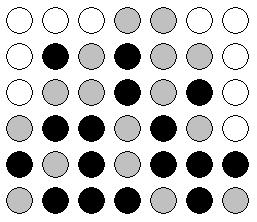
\includegraphics[width=0.8\textwidth]{image/puissance4}
		%\end{center}
		\end{minipage}
	%	&
		\begin{minipage}[t][][b]{10cm}
		N.B. : sur ce dessin noir et
		blanc, les jetons rouges apparaissent en noir, les jetons jaunes en
		gris et les cases blanches désignent l'absence de
		jetons. Cet exemple montre une situation du jeu où le joueur «~jaune~»
		est gagnant. En introduisant un jeton dans la
		4\textsuperscript{e} colonne,
		il a réalisé un alignement de 4 jetons en oblique.
		\end{minipage}
	%\end{supertabular}
	%\end{center}

	
	On demande d’implémenter une classe Puissance4 qui permette de contrôler
	l’état des différentes phases du jeu. Déterminez les attributs de cette
	classe et décrivez-les brièvement de manière à justifier votre choix.
	Dotez ensuite la classe des méthodes permettant de :

	\begin{liste}
		\item 
			savoir si la grille est pleine
		\item 
			mettre la grille à jour lorsque le joueur n (1 ou 2) joue dans la
			colonne j (entre 1 et 7). Cette méthode renverra la valeur booléenne
			faux si la colonne en question est déjà pleine
		\item 
			vérifier si le joueur qui vient de jouer dans la colonne j a gagné la
			partie
	\end{liste}
	
	N.B. : pour la structure qui contiendra le contenu du tableau de jetons,
	on adoptera la convention suivante : 0 pour l’absence de jeton, 1
	représentera un jeton du 1\textsuperscript{er} joueur, et 2 un jeton du
	2\textsuperscript{e} joueur (on peut donc faire abstraction de la
	couleur du jeton dans ce problème).
\end{Exercice}

\begin{Exercice}{Les congés}
	Les périodes de congés des différents employés d’une firme sont reprises
	dans un tableau booléen \textbf{Congés} bidimensionnel à \textit{n}
	lignes et 366 colonnes. Chaque ligne du tableau correspond à un employé
	et chaque colonne à un jour de l’année. Une case de ce tableau est mise
	à \textbf{vrai} si l’employé correspondant est en congé le jour
	correspondant. La firme en question est opérationnelle 7 jours sur 7,
	on n’y fait donc pas de distinction entre jours ouvrables, week-end et
	jours fériés.

	Ce tableau permet de visualiser l’ensemble des congés des travailleurs,
	et d’accorder ou non une demande de congé, suivant les règles suivantes :
	\begin{enumerate}
		\item 
			une période de congé ne peut excéder 15 jours ;
		\item 
			un employé a droit à maximum 40 jours de congé par an ;
		\item 
			à tout moment, 50\% des employés doivent être présents dans la firme.
	\end{enumerate}
	
	Écrire un algorithme qui détermine si cette demande peut être accordée
	ou non à un employé dont on connait le nom, ainsi que les dates de
	début et de fin d’une demande de congé (objets de la classe Date). Dans
	l’affirmative, le tableau \textbf{Congés} sera mis à jour.

	Pour établir la correspondance entre ce tableau et les noms des
	employés, vous avez à votre disposition un tableau \textbf{Personnel}
	de chaines. L’emplacement du nom d’un employé dans ce tableau
	correspond à l’indice ligne du tableau \textbf{Congés}.

	Il est permis d’utiliser pour résoudre cet exercice la méthode suivante
	de la classe Date, sans devoir détailler son code :
	
	\begin{Pseudocode}
		\MethodSign{numéroJour}{}{entier}
		\RComment la position du jour dans l’année (entre 1 et 366)
	\end{Pseudocode}
\end{Exercice}

\begin{Exercice}{L'ensemble}
		La notion d’ensemble fini est une notion qui vous est déjà 
		familière pour l’avoir rencontrée dans plusieurs cours. Nous rappelons
		certaines de ses propriétés et opérations. 
				
		Étant donnés deux ensembles
		finis \textbf{S} et \textbf{T} ainsi qu’un élément \textbf{x} :

		\begin{liste}
		\item 
			\textbf{x} {${\in}$} \textbf{S} signifie que l’élément \textbf{x}
			est un élément de l’ensemble \textbf{S}.
		\item 
			L’ensemble vide, noté \textbf{${\emptyset}$} 
			est l’ensemble qui n’a pas d’élément 
			(\textbf{x} {${\in}$} \textbf{${\emptyset}$} 
			est faux quel que soit \textbf{x} ).
		\item 
			L’ordre des éléments dans un ensemble n’a
			aucune signification, l’ensemble \{1,2\} est
			identique à \{2,1\}.
		\item 
			Un élément \textbf{x} ne peut
			pas être plus d’une fois élément d’un même ensemble 
			(pas de répétition).
		\item 
			L’union \textbf{S ${\cup}$ T} 
			est l’ensemble contenant les éléments qui sont dans 
			\textbf{S} ou (non exclusif) dans \textbf{T}.
		\item 
			L’intersection \textbf{S ${\cap}$ T} 
			est l’ensemble des éléments qui sont à la fois 
			dans \textbf{S} et dans \textbf{T}.
		\item 
			La différence \textbf{S {\textbackslash} T} 
			est l’ensemble des éléments qui sont 
			dans \textbf{S} mais pas dans \textbf{T}.
		\end{liste}
		
		Créer la classe \pseudocode{Ensemble}
		décrite ci-dessous.
		
		\begin{Pseudocode}
			\Class{Ensemble <T>}{} 
			\RComment T est le type des éléments de l'ensemble
			
				\Public
				\ConstrSign{Ensemble <T>}{} 
				\RComment construit un ensemble vide
				\MethodSign{ajouter}{élt : T}{}
				\RComment ajoute l'élément à l'ensemble
				\MethodSign{enlever}{élt : T}{})
				\RComment enlève un élément de l'ensemble
				\MethodSign{contient}{élt : T}{booléen}
				\RComment dit si l'élément est présent
				\MethodSign{estVide}{}{booléen}
				\RComment dit si l'ensemble est vide
				\MethodSign{taille}{}{entier}
				\RComment donne la taille de l'ensemble
				\MethodSign{union}{autreEnsemble : Ensemble <T>}{Ensemble <T>}
				\MethodSign{intersection}{autreEnsemble : Ensemble <T>}{Ensemble <T>}
				\MethodSign{moins}{autreEnsemble : Ensemble <T>}{Ensemble <T>}
				\MethodSign{listeÉléments}{}{Liste <T>}
				\RComment conversion en liste
			\EndClass
		\end{Pseudocode}
		
	\bigskip

	Quelques remarques :
	\begin{liste}
		\item 
			La méthode d'ajout (resp. de suppression) n'a
			pas d'effet si l'élément est déjà
			(resp. n'est pas) dans l'ensemble.
		\item 
			Les méthodes \pseudocode{union()}, 
			\pseudocode{intersection()} et 
			\pseudocode{moins()} retournent un troisième ensemble, 
			résultat des 2 premiers sans toucher
			à ces 2 ensembles. On aurait pu envisager des méthodes modifiant
			l'ensemble sur lequel on les appelle.
		\item 
			La méthode \pseudocode{listeÉlément()}
			est nécessaire si on veut parcourir les éléments de
			l'ensemble (par exemple pour les afficher).
	\end{liste}
	
	Autres opérations ensemblistes :
	Nous avons défini des opérations ensemblistes ne touchant pas aux
	ensembles de départ. Que deviennent-elles si on considère
	qu'elles \textbf{modifient}
	l'ensemble sur lequel elles sont appliquées ?
\end{Exercice}

\begin{Exercice}{Casino}
	Pour cet exercice,
	on vous demande un petit programme qui simule un jeu de roulette
	très simplifié dans un casino.
	
	Dans ce jeu simplifié, vous pourrez miser une certaine somme 
	et gagner ou perdre de l'argent (telle est la fortune, au casino !). 
	Quand vous n'avez plus d'argent, vous avez perdu.

	\textbf{Notre règle du jeu}

	Bon, la roulette, c'est très sympathique comme jeu, 
	mais un peu trop compliqué pour un exercice de première année.
	Alors, on va simplifier les règles et je vous présente tout de suite 
	ce que l'on obtient :
	\begin{liste}
	\item
		Le joueur mise sur un numéro compris entre 0 et 49 (50 numéros en tout). 
		En choisissant son numéro, il y dépose la somme qu'il souhaite miser.
	\item
		La roulette est constituée de 50 cases allant naturellement de 0 à 49. 
		Les numéros pairs sont de couleur noire, 
		les numéros impairs sont de couleur rouge. 
		Le croupier lance la roulette, 
		lâche la bille et quand la roulette s'arrête, 
		relève le numéro de la case dans laquelle la bille s'est arrêtée. 
		Dans notre programme, nous ne reprendrons pas tous ces détails 
		« matériels » mais ces explications sont aussi à l'intention 
		de ceux qui ont eu la chance d'éviter les salles de casino jusqu'ici. 
		Le numéro sur lequel s'est arrêtée la bille est, naturellement, 
		le numéro gagnant.
	\item
		Si le numéro gagnant est celui sur lequel le joueur a misé 
		(probabilité de 1/50, plutôt faible), 
		le croupier lui remet 3 fois la somme misée.
	\item
		Sinon, le croupier regarde si le numéro misé par le joueur 
		est de la même couleur que le numéro gagnant 
		(s'ils sont tous les deux pairs ou tous les deux impairs). 
		Si c'est le cas, le croupier lui remet 50\% de la somme misée. 
		Si ce n'est pas le cas, le joueur perd sa mise.
	\end{liste}
	
	Dans les deux scénarios gagnants vus ci-dessus 
	(le numéro misé et le numéro gagnant sont identiques ou ont la même couleur), 
	le croupier remet au joueur la somme initialement misée avant d'y ajouter ses gains. 
	Cela veut dire que, dans ces deux scénarios, le joueur récupère de l'argent. 
	Il n'y a que dans le troisième cas qu'il perd la somme misée. 
\end{Exercice}

\appendix
\chapter{Aide-mémoire}

Cet aide-mémoire peut vous accompagner lors d'une
interrogation ou d'un examen. Il vous est permis
d’utiliser ces classes et méthodes sans les développer.
Si vous sentez le besoin d’utiliser un objet ou une méthode qui
n'apparait pas ici, il faudra en écrire explicitement
le contenu et le code.

\section{Les caractères et les chaines}

\begin{Pseudocode}
	\Stmt {\large // Est-ce ?}
	\Empty
	\Stmt estLettre(car: caractère) \Gives~booléen		\RComment{est-ce une lettre ?}
	\Stmt estChiffre(car: caractère) \Gives~booléen		\RComment{est-ce un chiffre ?}
	\Stmt estMajuscule(car: caractère) \Gives~booléen	\RComment{est-ce une majuscule ?}
	\Stmt estMinuscule(car: caractère) \Gives~booléen	\RComment{est-ce une minuscule ?}
	\Empty
	\Stmt {\large // Conversions}
	\Empty
	\Stmt majuscule(car: caractère) \Gives~caractère	\RComment{convertit une minuscule en une majuscule.}
	\Stmt minuscule(car: caractère) \Gives~caractère	\RComment{convertit une majuscule en une minuscule.}
	\Stmt numLettre(car: caractère) \Gives~entier		\RComment{donne la position de la lettre dans l'alphabet.}
	\Stmt lettreMaj(n: entier) \Gives~caractère			\RComment{donne la lettre majuscule de position donnée.}
	\Stmt lettreMin(n: entier) \Gives~caractère			\RComment{donne la lettre minuscule de position donnée.}
	\Stmt chaine(car: caractère) \Gives~chaine			\RComment{convertit le caractère en une chaine.}
	\Let varChaine \Gets~varCaractère					\RComment{idem}
	\Stmt chaine(n : entier) \Gives~chaine				\RComment{convertit un entier en une chaine.}
	\Stmt chaine(x : réelr) \Gives~chaine				\RComment{convertit un réel en une chaine.}
	\Stmt nombre(ch : chaine) \Gives~réel				\RComment{convertit une chaine en un nombre.}
	\Empty
	\Stmt {\large // Manipulations}
	\Empty
	\Stmt longueur(ch : chaine) \Gives~entier			\RComment{donne la taille de la chaine.}
	\Stmt car(ch: chaine, n: entier) \Gives~caractère	\RComment{donne le caractère à une position donnée.}
	\Stmt sousChaine(ch: chaine, pos: entier, long: entier) \Gives~chaine \RComment{extrait une sous-chaine}
	\Stmt estDansChaine(ch: chaine, sous-chaine: chaine [ou caractère]) \Gives~entier 
	\Stmt 	\RComment{dit où commence une sous-chaine dans une chaine donnée (0 si pas trouvé)}
	\Stmt concat(ch1, ch2, \dots, chN: chaine) \Gives~chaine 	\RComment{concatène des chaines}
	\Let  ch \Gets~ch1 + ch2 + \dots + chN						\RComment{idem}
\end{Pseudocode}

\section{La liste}

\begin{Pseudocode}
\Class{Liste <T>}
\Public
	\ConstrSign{Liste <T>}{} 
	\MethodSign{get}{pos : entier}{T} \RComment retourne l’élément en position pos
	\MethodSign{set}{pos : entier, valeur : T}{} \RComment modifie l’élément en position pos
	\MethodSign{taille}{}{entier} \RComment retourne la taille de la liste
	\MethodSign{ajouter}{valeur : T}{} \RComment ajoute une valeur en fin de liste
	\MethodSign{insérer}{pos : entier, valeur : T}{} \RComment insère un élément en position pos
	\MethodSign{supprimer}{}{} \RComment supprime le dernier élément
	\MethodSign{supprimerPos}{pos : entier}{} \RComment supprime l’élément en position pos
	\MethodSign{supprimer}{valeur : T}{} \RComment supprime l’élément de valeur donnée
	\MethodSign{vider}{}{} \RComment vide la liste
	\MethodSign{estVide}{}{booléen} \RComment indique si la liste est vide
	\MethodSign{existe}{valeur\In : T, pos\Out : entier}{booléen} \RComment recherche un élément
\EndClass
\end{Pseudocode}

\section{Date, Moment, Durée}

\begin{Pseudocode}
\Class{Date}
\Public
	\ConstrSign{Date}{} \RComment Crée la date du jour
	\ConstrSign{Date}{j, m, a : entiers} 
	\MethodSign{getJour}{}{entier}
	\MethodSign{getMois}{}{entier}
	\MethodSign{getAnnée}{}{entier}
	\MethodSign{égale}{autreDate : Date}{booléen}
	\MethodSign{estAntérieure}{autreDate : Date}{booléen}
\EndClass
\end{Pseudocode}

\begin{Pseudocode}
\Class{Moment}
\Public
	\ConstrSign{Moment}{} \RComment Crée le moment courant
	\ConstrSign{Moment}{h, m, s : entiers} 
	\MethodSign{getHeure}{}{entier}
	\MethodSign{getMinute}{}{entier}
	\MethodSign{getSeconde}{}{entier}
	\MethodSign{setHeure}{h : entier}{}
	\MethodSign{setMinute}{m : entier}{}
	\MethodSign{setSeconde}{s : entier}{}
	\MethodSign{égal}{autreMoment : Moment}{booléen}
	\MethodSign{estAntérieur}{autreMoment : Moment}{booléen}
\EndClass
\end{Pseudocode}

\begin{Pseudocode}
\Class{Durée}
\Public
	\ConstrSign{Durée}{secondes : entier} 
	\ConstrSign{Durée}{h, m, s : entiers} 
	\MethodSign{getJour}{}{entier}
	\MethodSign{getHeure}{}{entier}
	\MethodSign{getMinute}{}{entier}
	\MethodSign{getSeconde}{}{entier}
	\MethodSign{getTotalHeure}{}{entier}
	\MethodSign{getTotalMinute}{}{entier}
	\MethodSign{getTotalSeconde}{}{entier}
	\MethodSign{ajouter}{autreDurée : Durée}{}
	\MethodSign{soustraire}{autreDurée : Durée}{}
	\MethodSign{égale}{autreDurée : Durée}{booléen}
	\MethodSign{plusPetit}{autreDurée : Durée}{booléen}
\EndClass
\end{Pseudocode}


% Une méthode égale pour tous.
% ajouter valeurAbsolue(entier)


%\printindex
%\addcontentsline{toc}{chapter}{Index}

\end{document}
